\documentclass[11pt,aspectratio=169]{beamer}
%\documentclass[11pt,aspectratio=169, handout]{beamer}
%\usepackage{handoutWithNotes}
\usetheme[outer/progressbar=foot,
%outer/numbering=none
]{metropolis}
\setbeamertemplate{caption}{\raggedright\insertcaption\par}
\setbeamercolor{frametitle}{bg={}, fg=black!80}
\definecolor{myorange}{rgb}{0.8500, 0.3250, 0.0980}
\setbeamercolor{alerted text}{bg={}, fg=myorange }
\setbeamercolor{block title}{bg=black!10, fg=black}
\setbeamercolor{block body}{bg=black!10, fg=black}
\setbeamercolor{block frame}{bg=black, fg=black}
\setbeamertemplate{blocks}[rounded]
\setbeamertemplate{blocks}[framed]
%\usecolortheme{seahorse}
\usepackage[utf8]{inputenc}
\usepackage[english]{babel}
%\usepackage[T1]{fontenc}
\newcommand{\tr}[1]{\textcolor{blue}{#1}}
\usepackage{amsmath}
\usepackage{amsfonts}
\usepackage{amssymb}
\usepackage{mathtools}
\usepackage{calc}
\usepackage{soul}
\setbeamercolor{headerCol}{fg=blue!30,bg=black!80}
\setbeamercolor{bodyCol}{fg=black}
\usepackage{graphicx}
\usepackage{xcolor}
\usepackage{appendix}
\usepackage{hyperref}
\usepackage{natbib}
\usepackage{comment}
\usepackage{setspace}
\renewcommand{\bibsection}{}
\bibliographystyle{apa} 
% have to run bibtex mydocument.aux after first run to generate bbl file. 
\usepackage{appendixnumberbeamer}
\usepackage{xcolor}

%table
\usepackage{makecell}
\usepackage{multirow}
\usepackage{bigdelim}

\usepackage[customcolors]{hf-tikz}
\definecolor{sonja}{cmyk}{1.5,0,0.9,0.3}
%\definecolor{blue}{cmyk}{0,1,0,0}
\hfsetfillcolor{black!10}
\hfsetbordercolor{black}

\usepackage{tikz}
\usetikzlibrary{tikzmark}
\usetikzlibrary{decorations.markings}
\usepackage{tikz-cd}
\usetikzlibrary{arrows,calc,fit}
\tikzset{mainbox/.style={draw=white, text=white, fill=gray, rectangle, rounded corners, thick, node distance=7em, text width=8em, text centered, minimum height=3.5em}}
\tikzset{dummybox/.style={draw=none, text=white , rectangle, rounded corners, thick, node distance=7em, text width=8em, text centered, minimum height=3.5em}}
\tikzset{box/.style={draw , rectangle, rounded corners, thick, node distance=7em, text width=8em, text centered, minimum height=3.5em}}
\tikzset{container/.style={draw, rectangle, dashed, inner sep=2em}}
\tikzset{line/.style={draw, very thick, -latex'}}
\tikzset{    pil/.style={
		->,
		thick,
		shorten <=2pt,
		shorten >=2pt,}}
\tikzstyle{vecArrow} = [thick, decoration={markings,mark=at position
	1 with {\arrow[semithick]{open triangle 60}}},
double distance=1.4pt, shorten >= 5.5pt,
preaction = {decorate},
postaction = {draw,line width=1.4pt, white,shorten >= 4.5pt}]


%TITLE
\author[Sonja Dobkowitz]{\small Sonja Dobkowitz\\ \footnotesize{University of Bonn%, RTG 2281 The Macroeconomics of Inequality}
	}\\ }
%\institute[University of Bonn]{}
\title{The role of fiscal policies in meeting climate targets}

\newcommand{\ar}{$\Rightarrow$ \ }

%\addtobeamertemplate{navigation symbols}{}{%
%    \usebeamerfont{footline}%
%    \usebeamercolor[fg]{footline}%
%    \hspace{1em}%
%   \insertframenumber/\inserttotalframenumber
%}

%\institute{University of Bonn} 
\date{\small{RTG Retreat\\ June 12, 2022 }} 
%\subject{} 
\begin{document}
	
	{\setbeamertemplate{footline}{}
		\begin{frame}
		\titlepage
	\end{frame}
}
%\addtocounter{framenumber}{-1}

% {\setbeamertemplate{footline}{}
% \begin{frame}{Content}
% \vspace{4mm}
% \tableofcontents
% \end{frame}
% }
 %\addtocounter{framenumber}{-1}


%---------------------------------------
%            Intro
%---------------------------------------
%\section{ Reducing Consumption Levels}
\addtocounter{framenumber}{-1}
\begin{frame}{Motivation}

\begin{itemize}[<+-| alert@+>]
	\setbeamercolor{alerted text}{} %change the font color
	\setbeamerfont{alerted text}{}
%	\item we are facing  environmental limits 
%	\vspace{3mm}
	\item 	natural scientists suggest stricter emission limits to meet temperature targets \\ \small{(Intergovernmental Panel on Climate Change \citep{Rogelj2018MitigationDevelopment., IPCC2022})}
\vspace{3mm}
	\item some scholars argue for \textit{reductive policies} to handle environmental limits\\ \small{\citep{Schor2005SustainableReduction, Arrow2004AreMuch, Dasgupta2021}}
	\vspace{3mm}
	\item but: models on optimal environmental policy abstract from reductive policy tools % (e.g. distortionary fiscal policies)% inelastic labour supply, no income tax
	\vspace{3mm}
\item \textbf{Can fiscal policies help meet emission limits?}
\end{itemize}
\end{frame}

%\begin{frame}{Trade-offs}
%	\textbf{Starting from demand target}
%\begin{itemize}
%\item lowering demand for certain land and energy-intense products could be regressive but natural scientists call for such a reduction in demand to meet climate targets
%\item labour income taxation could be an alternative measure/ potentially less politically debated
%\item However, new trade-offs arise from a higher tax progressivity: 
%\begin{enumerate}
%	\item on the one hand, it lowers demand, on the other hand, it could imply a shift to dirty innovations and production through a skill-bias mechanism \ar a new equity-environment trade-off arises
%	\item the progressivity of the tax system affects the composition of aggregate demand: if the rich have a higher propensity to consume clean, it raises pollution
%\end{enumerate}
%\item if inequality suffers, look at alternative measure of lowering hours worked
%\item on the other hand, fossil taxes counter equity if they foster skill bias of innovations
%\end{itemize}
%\end{frame}
%\begin{frame}{Working hypotheses}	
%	\begin{enumerate}
%		\item<+-> with short time until growth in fossil sector has to stop, green innovation rate could be too slow to only rely on fossil taxes and subsidies \ar role for fiscal policies (demand reduction policies) \ar progressive tax
%		\vspace{3mm}
%		\item<+-> Skill heterogeneity and skill-bias in green sector make a regressive tax optimal to subsidise green innovations
%		\vspace{3mm}
%		\item<+-> income-dependent marginal propensities to consume emissions make a a \textbf{higher progressivity} optimal if the rich have a higher marginal propensity to consume green (MPCG); and a \textbf{more regressive income} tax is optimal if the poor have a higher MPCG (need to include inequality) 
%		\vspace{3mm}
%		\item<+-> now households are willing to reduce their consumption deliberately: reduction in satiation point; of high energy goods only, meat etc. 
%		%\item<+-> could also have motive to reduce demand due to short time frame until emissions have to be zero and a too slow innovation rate (look at model without skill heterogeneity)
%	\end{enumerate}
%\end{frame}

\begin{frame}{This paper}
	\begin{itemize}
		\item<+-> quantitative \alert{endogenous growth} model building on \cite{Fried2018ClimateAnalysis}
		\vspace{3mm}
		\item<+->  \alert{emission limit constraints} the government when  {maximising social welfare}
		\vspace{3mm}
		\item<+-> the government can use \alert{fossil} and \alert{distortionary income taxes}
		\vspace{3mm}
		%	\item<+-> profitability of research in each sector determines sector growth
		\item<+->  \alert{representative} household  
		\vspace{2mm}
		\begin{itemize}
			\item[-]<+->\alert{elastic} labour supply \ar \textit{reductive effect} of income tax
			\vspace{2mm}
			\item[-]<+->  \alert{low and high skill} \ar \textit{recomposing effect} of income tax:\\ \hspace{32mm} green sector is skill-biased  \small{\citep{Consoli2016DoCapital}}
		\end{itemize}
		
		%	\vspace{3mm}
		%	\item<+-> the government chooses fossil and distortionary income taxes
		%	\vspace{3mm}
		%\item<+-> in an extension: Households voluntarily reduce consumption and labour supply
		% as households reduce consumption themselves, (1) less need for reduction polices, (2) lower inefficiency through skill recomposition 
	\end{itemize}
\end{frame}
%\addtocounter{framenumber}{-1}
%\begin{frame}{This paper}
%	\begin{itemize}
%		\item quantitative \alert{endogenous growth} model building on \cite{Fried2018ClimateAnalysis}
%		\vspace{3mm}
%		\item  \alert{emission limit constraints} the government when  {maximising social welfare}
%		\vspace{3mm}
%		\item the government can use \alert{fossil} and \alert{distortionary income taxes}
%		\vspace{3mm}
%		%	\item<+-> profitability of research in each sector determines sector growth
%		\item  representative household \alert{elastically} supplies labour of two types: low- and high-skilled
%		\vspace{2mm}
%		\begin{itemize}
%			\item[-]<+-> \textit{reductive effect} of income tax
%			\vspace{1mm}
%			\item[]%<+-> %\textit{recomposing effect} of income tax: green sector is skill-biased  \citep{Consoli2016DoCapital}
%		\end{itemize}
%		
%		%	\vspace{3mm}
%		%	\item<+-> the government chooses fossil and distortionary income taxes
%		%	\vspace{3mm}
%		%\item<+-> in an extension: Households voluntarily reduce consumption and labour supply
%		% as households reduce consumption themselves, (1) less need for reduction polices, (2) lower inefficiency through skill recomposition 
%	\end{itemize}
%\end{frame}
%\addtocounter{framenumber}{-1}
%\begin{frame}{This paper}
%\begin{itemize}
%	\item quantitative \alert{endogenous growth} model building on \cite{Fried2018ClimateAnalysis}
%	\vspace{3mm}
%	\item  \alert{emission limit constraints} the government when  {maximising social welfare}
%	\vspace{3mm}
%	\item the government can use \alert{fossil} and \alert{distortionary income taxes}
%	\vspace{3mm}
%	%	\item<+-> profitability of research in each sector determines sector growth
%	\item  representative household {elastically} supplies labour \alert{of two types: low- and high-skilled } 
%	\vspace{2mm}
%	\begin{itemize}
%		\item[-] \textit{reductive effect} of income tax
%		\vspace{1mm}
%		\item[-]<+-> \textit{recomposing effect} of income tax: green sector is skill-biased  \citep{Consoli2016DoCapital}
%	\end{itemize}
%	
%%	\vspace{3mm}
%%	\item<+-> the government chooses fossil and distortionary income taxes
%%	\vspace{3mm}
%%\item<+-> in an extension: Households voluntarily reduce consumption and labour supply
%% as households reduce consumption themselves, (1) less need for reduction polices, (2) lower inefficiency through skill recomposition 
%\end{itemize}
%\end{frame}

%\begin{frame}{How}
%	\begin{itemize}
%		\item<+-> the emission target determines fossil output starting from 2050
%		\vspace{3mm}
%		\item<+-> model economy on BGP (with constant growth ratios) until today; then, allow for non-balanced trajectory under optimal policy
%		\vspace{3mm}
%		\item<+-> first pass: starting in 2020, the planner optimises over a \textbf{finite horizon} only (political economy argument), and has to meet emission target (adapt code in \cite{Barrage2019OptimalPolicy})
%	\end{itemize}
%\end{frame}

\begin{frame}{Preview of results}
	\pause
\begin{enumerate}
	\item<+-> the \alert{optimal income tax is progressive}  to reduce inefficiently high hours worked
	\vspace{5mm}
	\item<+->  meeting the emission limit is mainly accounted for by the fossil tax
	\vspace{5mm}
	\item<+-> the use of income taxes \alert{raises social welfare by 0.11\%}   %but are nnot necessary to meet the emission limit %
	from 2020 to 2080 \\ \small{(without  skill heterogeneity by 0.85\%)}
	
	\vspace{5mm}
	%\item<+->  \alert{sizable effect of skill heterogeneity}: \\ with only one skill, the optimal income tax increases social welfare by 0.85\%
\end{enumerate}
\end{frame}
%\begin{frame}{Roadmap}
%	\tableofcontents
%\end{frame}

\section{Model}

\begin{comment}
\begin{frame}{Model Overview}
	
	\centering
	\resizebox{0.9\textwidth}{!}{
		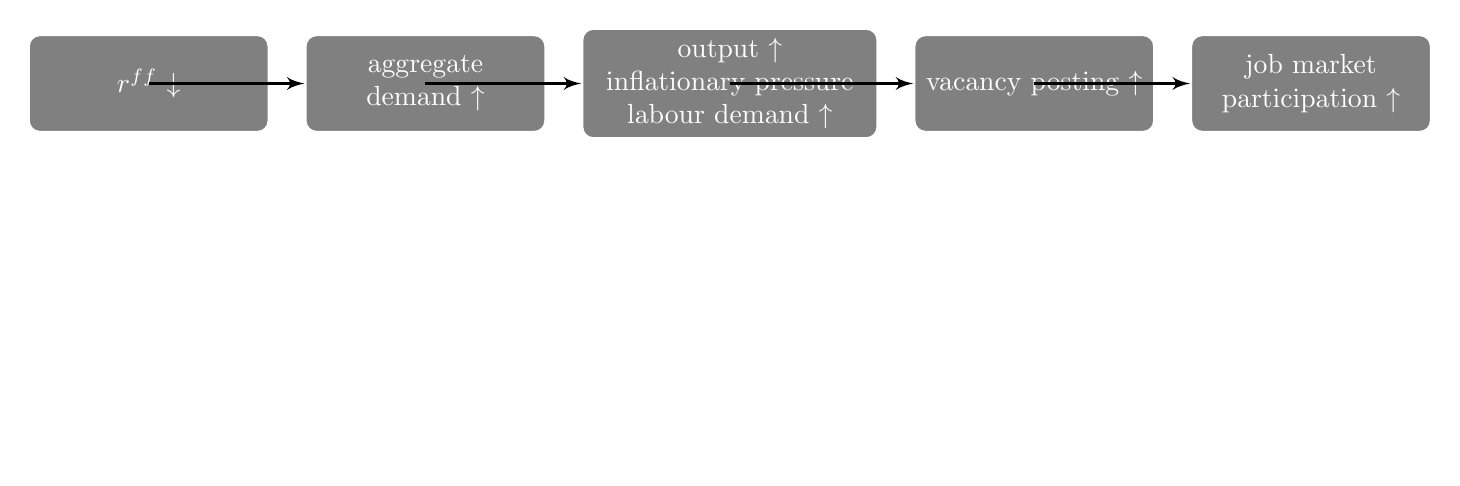
\begin{tikzpicture}[  yshift=.25\baselineskip]
		\node [mainbox] (ffr) {$r^{ff}$ \textbf{$\downarrow$}};
		<-2>\node [mainbox, right of=ffr, node distance =10em] (aggdem) {aggregate demand $\uparrow$};
		\node [mainbox, right of=aggdem , node distance =11em, text width=10em] (output) {output $\uparrow$\\ inflationary pressure \\ labour demand $\uparrow$};
		\node [mainbox, right of=output , node distance =11em] (vacancies) {vacancy posting $\uparrow$};
		\node [mainbox, right of=vacancies , node distance =10em] (participation) {job market \\participation $\uparrow$};
		
		\coordinate (middle) at ($(vacancies.south)!0.5!(participation.south)$);
	%	\coordinate (mid) at ($(ffr.east)!0.5!(spread.west)$);
		
		\node [dummybox, below of=middle , node distance =10em, text width =15em] (sam_eff) {};
		
		
		\coordinate (left_sam) at ($(sam_eff.north)!0.5!(middle.north)$);
		
		\node [dummybox, left of=left_sam , node distance =10em,] (sam_eff) {};
		
		%actors
		% \node [box, above of=left, node distance =4em] (banks) {Banks' market power };
		% \node [mainbox, below of=middle, node distance =5em] (loans) { bank new portfolio (long-term) lending $\downarrow $ };
		
		\path [line] (ffr) |- (aggdem);
		\path [line] (aggdem) |- (output);
		\path [line] (output) |- (vacancies);
		\path [line] (vacancies) |- (participation);
		
		% \path [line](depos)|- (loans.east);
		% \draw [->, very thick]  (banks) -- (left);
		
		% \node[mainbox, right of=loans, node distance =14em] (PLSbank) {PLS lending $\uparrow$};
		
		% \path [line](depos)|- (PLSbank.west);
		
		\end{tikzpicture}
		
	}
\end{frame}
	content...
\end{comment}
%\begin{comment}
\begin{frame}{Model overview}

	\vspace{-2mm}
	\begin{enumerate}
		\item<+-> \textbf{representative household} supplies high and low-skilled labour and consumes 

		 \vspace{2mm}
		 
		\item<+-> \textbf{production}
		\begin{itemize}
			\item<+-> competitive final good producers ($Y$)
			\item<+-> non-energy ($N$) and energy producers ($ E$)
			\item<+-> fossil and green energy producers ($F,G$)
			\item<+-> labour input good producers ($h_h, h_l \rightarrow L_f, L_g, L_n$)
			\item<+-> monopolistically competitive machine producers ($x_n, x_f, x_g$)
		\end{itemize}
		\vspace{2mm}
		\item<+-> \textbf{research}
		\begin{itemize}
			\item<+-> machine producers (demand research)
			\item<+-> scientists (supply research)
		\end{itemize}
		\item<+-> \textbf{government} %seeks to maximise social welfare but is constrained by an emission limit
	\end{enumerate} 
\end{frame}

%content...
%\end{comment}

\begin{frame}{Household}
\hypertarget{backhh}{}
%\text{\textbf{Householdrt}}
\vspace{2mm}
\begin{minipage}[t!]{1\textwidth}
	\begin{align*}
	\tikzmarkin{first}(1.5,3.4)(-1.2,-2.7)
	%	\underset{c_{s,i},c_{n,i}, l_i}{\max} \ \hspace{2mm} U(c_{s,i}, c_{n,i}, l_i; h_n)= 
 \max_{\{C_t\}_{t=0}^\infty, \{h_{ht}\}_{t=0}^\infty, \{h_{lt}\}_{t=0}^\infty} \sum_{t=0}^\infty \beta^t \left(\log(C_t)-z_h\chi\frac{h_{ht}^{1+\sigma}}{1+\sigma}-(1-z_h)\chi\frac{h_{lt}^{1+\sigma}}{1+\sigma}\right) %when z is also to the power of 1+sigma than, the higher zh the lower hours supplied! Not reasonable
\\
\vspace{4mm}
\\
s.t.\ C_t=z_h \alert{\pmb{\lambda_t}} (w_{ht}h_{ht})^{\alert{\pmb{1-\tau_{\iota t}}}}+(1-z_h) \pmb{\alert{\lambda_t}} (w_{lt}h_{lt})^{\alert{\pmb{1-\tau_{\iota t}}}}%+Gov_t
\\
\hspace{2mm}\ h_{ht}\leq \bar{H}; \hspace{4mm} h_{lt}\leq \bar{H}
	\tikzmarkend{first}
	\end{align*}
\end{minipage}

%\begin{minipage}[t!]{0.4\textwidth}
%
%\begin{align*}
%\hspace{4mm}c =
%\left(\textcolor{blue}{\omega}^{\frac{1}{\sigma}}c_{s}^{\frac{\sigma-1}{\sigma}}+(1-\textcolor{blue}{\omega})^{\frac{1}{\sigma}}c_{n}^{\frac{\sigma-1}{\sigma}}\right)^{\frac{\sigma}{\sigma-1}}& \hspace{2mm} \text{where} \hspace*{2mm} \sigma \neq 1
%\end{align*}
%\end{minipage}

\small
\vspace{4mm}
\begin{minipage}[t!]{0.4\textwidth}
	\vspace{7mm}
	\begin{itemize}
		\item[] $z_h$:\ \ share of high-skilled labour \vspace{-2mm}
		\item[] $h_{ht}$: hours high skilled\vspace{-2mm}
		\item[] $h_{lt}$:\ \ hours low skilled\vspace{-2mm}
%		\item[] $S_{t}$:\ \  \ hours scientists\vspace{-2mm}
	\end{itemize}
\end{minipage}
\begin{minipage}[t!]{0.5\textwidth}
	\vspace{8mm}
	\begin{itemize}
		\item[] $\tau_{\iota t}$: income tax progressivity \vspace{-2mm}
		\item[] \ \ \ \ \  $\tau_{\iota t}>0$ \ar progressive tax
		\vspace{-2mm}	
		\item[] $\lambda_{t}$: shifts average tax payments
%		\vspace{-2mm}	
%		\item[]%	$Gov_{t}$: government transfers
	\end{itemize}
\end{minipage}


\vspace{4mm}
\hfill
\hyperlink{taxsc}{\tiny{$\rightarrow$ tax scheme,}} \hyperlink{opth}{\tiny{$\rightarrow$ optimal labour supply,}} 
\hyperlink{skillr}{\tiny{$\rightarrow$ skill ratio}}
\end{frame}

\begin{frame}{ Production}
\textbf{Final good and energy producers }
\vspace{-5mm}
	\begin{minipage}[t!]{1\textwidth}
		\begin{align*}
		\tikzmarkin{second}(1.3,1.2)(-1,-0.8)
Y_t=\left(\delta_y^{\frac{1}{\varepsilon_y}}E_t^\frac{\varepsilon_y-1}{\varepsilon_y}+(1-\delta_y)^{\frac{1}{\varepsilon_y}}N_t^\frac{\varepsilon_y-1}{\varepsilon_y}\right)^\frac{\varepsilon_y}{\varepsilon_y-1}; \ \ 
E_t=\left({F}_t^\frac{\varepsilon_e-1}{\varepsilon_e}+G_t^\frac{\varepsilon_e-1}{\varepsilon_e}\right)^\frac{\varepsilon_e}{\varepsilon_e-1}
\tikzmarkend{second}
\end{align*}
	\end{minipage}
\pause
\\

\vspace{12mm}
\textbf{Non-energy, fossil, and green energy producers:} $J\ \in\{F,G,N\}$
%\pause
	\vspace{-3mm}
\begin{minipage}[t!]{1\textwidth}
	\begin{align*}
	\tikzmarkin{third}(7.8,2.8)(-2.8,-2.3)
\underset{\{x_{ijt}\}_{i=0}^1, L_{jt}}{\max}\ & \pi_{jt}=\textcolor{black!10}{(1-{\pmb{\tau_{jt}}})}p_{jt}J_t-w_{ljt}L_{jt}-\int_{0}^{1}p_{ijt}x_{ijt}di\\ 
 s.t.\ & J_{t}=L_{jt}^{1-\alpha_j}\int_{0}^{1}A^{1-\alpha_j}_{ijt}x_{ijt}^{\alpha_j}di \\
 \ & \textcolor{black!10}{\tau_{nt}=\tau_{gt}=0}
	\tikzmarkend{third}
	\end{align*}
\end{minipage}
\end{frame}

\addtocounter{framenumber}{-1}
\begin{frame}{ Production}
	\textbf{Final good and energy producers }
	\vspace{-5mm}
	\begin{minipage}[t!]{1\textwidth}
		\begin{align*}
		\tikzmarkin{second}(1.3,1.2)(-1,-0.8)
		Y_t=\left(\delta_y^{\frac{1}{\varepsilon_y}}E_t^\frac{\varepsilon_y-1}{\varepsilon_y}+(1-\delta_y)^{\frac{1}{\varepsilon_y}}N_t^\frac{\varepsilon_y-1}{\varepsilon_y}\right)^\frac{\varepsilon_y}{\varepsilon_y-1}; \ \ 
		E_t=\left({F}_t^\frac{\varepsilon_e-1}{\varepsilon_e}+G_t^\frac{\varepsilon_e-1}{\varepsilon_e}\right)^\frac{\varepsilon_e}{\varepsilon_e-1}
		\tikzmarkend{second}
		\end{align*}
	\end{minipage}
	\\
	
	\vspace{12mm}
	\textbf{Non-energy, fossil, and green energy producers:} $J\ \in\{F,G,N\}$
	%\pause
	\vspace{-3mm}
	\begin{minipage}[t!]{1\textwidth}
		\begin{align*}
		\tikzmarkin{third}(6.8,2.2)(-1.8,-2)
		\underset{\{x_{ijt}\}_{i=0}^1, L_{jt}}{\max}\ & \pi_{jt}=(1-\alert{\pmb{\tau_{jt}}})p_{jt}J_t-w_{ljt}L_{jt}-\int_{0}^{1}p_{ijt}x_{ijt}di \hspace{3mm} \pmb{\alert{for\  J=F}}\\ 
		s.t.\ & J_{t}=L_{jt}^{1-\alpha_j}\int_{0}^{1}A^{1-\alpha_j}_{ijt}x_{ijt}^{\alpha_j}di
%		 \\
%		\ & \tau_{nt}=\tau_{gt}=0
		\tikzmarkend{third}
		\end{align*}
	\end{minipage}
\end{frame}

\begin{frame}{ Labour and machines}
	
	\textbf{Labour input good producers:} $J\ \in\{F,G,N\}$\\ \vspace{0mm}
	\begin{minipage}[t!]{1\textwidth}
		\begin{align*}
		\tikzmarkin{fourth}(5.8,1)(-5.6,-0.6)
		 L_{jt}=h_{hjt}^{\theta_{j}}h_{ljt}^{1-\theta_{j}}
		\tikzmarkend{fourth}
		\end{align*}
	\end{minipage}
\\
\pause

\vspace{7mm}
	\textbf{Monopolistically competitive machine producers }\\ \vspace{-1mm}
\begin{minipage}[t!]{1\textwidth}
	\begin{align*}
	\tikzmarkin{sixth}(6.3,4)(-2.7,-3.8)
\underset{p_{xijt}, s_{jit}}{\max}\ & p_{xijt}(1+\zeta_{jt})x_{ijt}-x_{ijt}-w_{sjt}s_{ijt}\\
s.t.\ &(1)\ \text{demand for machines }\\ %x_{ijt}= \left(\frac{p_{ft}(1-\tau_{jt})\alpha_j}{p_{xijt}}\right)^\frac{1}{1-\alpha_j}A_{ijt}L_{jt}\\
& \textcolor{black!10}{(2)\ A_{ijt}=A_{jt-1}\left(1+\gamma\left(\frac{s_{ijt}}{\rho_j}\right)^\eta\left(\frac{A_{t-1}}{A_{jt-1}}\right)^\phi\right)}\\
& \textcolor{black!10}{\text{where}\ \ \ A_{jt}=\int_{0}^{1}A_{ijt} di}
	\tikzmarkend{sixth}
	\end{align*}
\end{minipage}
\end{frame}

\addtocounter{framenumber}{-1}

\begin{frame}{ Labour and machines}
	
	\textbf{Labour input good producers:} $J\ \in\{F,G,N\}$\\ \vspace{0mm}
	\begin{minipage}[t!]{1\textwidth}
		\begin{align*}
		\tikzmarkin{fourth}(5.8,1)(-5.6,-0.6)
		L_{jt}=h_{hjt}^{\theta_{j}}h_{ljt}^{1-\theta_{j}}
		\tikzmarkend{fourth}
		\end{align*}
	\end{minipage}
	\\
	
	\vspace{7mm}
	\textbf{Monopolistically competitive machine producers }\\ \vspace{-1mm}
	\begin{minipage}[t!]{1\textwidth}
		\begin{align*}
		\tikzmarkin{sixth}(6.3,4)(-2.7,-3.8)
		\underset{p_{xijt}, s_{jit}}{\max}\ & p_{xijt}(1+\zeta_{jt})x_{ijt}-x_{ijt}-w_{sjt}s_{ijt}\\
		s.t.\ &(1)\ \text{demand for machines }\\ %x_{ijt}= \left(\frac{p_{ft}(1-\tau_{jt})\alpha_j}{p_{xijt}}\right)^\frac{1}{1-\alpha_j}A_{ijt}L_{jt}\\
		& {(2)\ A_{ijt}=A_{jt-1}\left(1+\gamma\left(\frac{s_{ijt}}{\rho_j}\right)^\eta\left(\frac{A_{t-1}}{A_{jt-1}}\right)^\phi\right)}\\
		& {\text{where}\ \ \ A_{jt}=\int_{0}^{1}A_{ijt} di}
		\tikzmarkend{sixth}
		\end{align*}
	\end{minipage}
\end{frame}
%\begin{frame}{Model: Machine Producers and Innovation}
%
%\textbf{Marginal product of innovation}
%\begin{align*}
%&
%w_{sjt}=\frac{\eta \gamma \alpha_f A_{jt-1}^{1-\phi}A_{t-1}^{\phi}\left(\frac{S_{jt}}{\rho_j}\right)^{\eta}p_{jt}J_t}{\frac{1}{1-\alpha_f}S_{jt}A_{jt}}\\
%\end{align*}
%\end{frame}

\begin{frame}{ Scientists and markets}
\textbf{Scientists}\\
\vspace{2mm}
\begin{minipage}[t!]{1\textwidth}
	\begin{align*}
	\tikzmarkin{seventh}(6.7,2)(-5,-1.2)
\underset{s_{jt}}{\max}\ \ & w_{jst}s_{jt}-\chi_s \frac{s_{jt}^{1+\sigma_s}}{1+\sigma_s}\\
s.t. \ \ & s_{jt}\leq \bar{H}	\tikzmarkend{seventh}
	\end{align*}
\end{minipage}
\\
\pause

\vspace{9mm}
\textbf{Markets}\\ \vspace{1mm}
\begin{minipage}[t!]{1\textwidth}
	\begin{align*}
	\tikzmarkin{8th}(3.6,2.4)(-4.5,-2.2)
z_h h_{ht}&=h_{hft}+h_{hgt}+h_{hnt}\\
(1-z_h) h_{lt}&=h_{lft}+h_{lgt}+h_{lnt}\\
C_t&=Y_t-\int_{0}^{1}\left(x_{fit}+x_{git}+x_{nit}\right)di
	\tikzmarkend{8th}
	\end{align*}
\end{minipage}
\end{frame}

\begin{frame}{ Government}
	\begin{minipage}[t!]{1\textwidth}
		\begin{align*}
		\tikzmarkin{9th}(9.7,4.5)(-1.3,-4)
		&\max_{\{\tau_{ft}\}_{t=0}^{T}, \{\tau_{\iota t}\}_{t=0}^{T}} \sum_{t=0}^{T}\beta^t U_{t}\\
	\textcolor{black!10}{s.t.} \hspace{4mm}
		&\textcolor{black!10}{ (1)\ \ T_t= z_h(w_{ht}h_{ht}-\lambda_t(w_{ht}h_{ht})^{{\pmb{1-\tau_{\iota t}}}})+(1-z_h)(w_{ht}h_{ht}-\lambda_t(w_{ht}h_{ht})^{{\pmb{1-\tau_{\iota t}}}})}\\ & \hspace{15mm } \textcolor{black!10}{+{\pmb{\tau_{ft}}}p_{ft}F_{t}}\\
		& \textcolor{black!10}{(2)\ \text{behaviour of firms, scientists, and households}}\\
		& \textcolor{black!10}{(3)\ \text{feasibility} }\\
		&\textcolor{black!10}{
			(2)\ \  \omega F_t-\delta =\Omega_t }
		\tikzmarkend{9th}
		\end{align*}
	\end{minipage}
	
	\small
	\vspace{0mm}
	\begin{minipage}[t!]{0.35\textwidth}
		\vspace{7mm}
		\begin{itemize}
			\item[] %$T_t$: transfers, set to zero  \vspace{0mm}
			%	\item[] $\delta$: carbon sinks\vspace{-2mm}
			\item[] 
		\end{itemize}
	\end{minipage}
	\begin{minipage}[t!]{0.6\textwidth}
		\vspace{8mm}
		\begin{itemize}
			\item[]% $\Omega_{t}$: exogenous emission limit
			\vspace{0mm}	
			\item[] %$\omega$:\ \ $CO_2$ equivalent emissions \\ \hspace{4mm} per unit of fossil energy
		\end{itemize}
	\end{minipage}
\end{frame}
\addtocounter{framenumber}{-1}
\begin{frame}{Model: Government}
	\begin{minipage}[t!]{1\textwidth}
		\begin{align*}
		\tikzmarkin{9th}(9.7,4.5)(-1.3,-4)
		&\max_{\{\tau_{ft}\}_{t=0}^{T}, \{\tau_{\iota t}\}_{t=0}^{T}} \sum_{t=0}^{T}\beta^t U_{t}\\
		s.t. \hspace{4mm}
		&(1)\ \ T_t= z_h(w_{ht}h_{ht}-\lambda_t(w_{ht}h_{ht})^{\alert{\pmb{1-\tau_{\iota t}}}})+(1-z_h)(w_{ht}h_{ht}-\lambda_t(w_{ht}h_{ht})^{\alert{\pmb{1-\tau_{\iota t}}}})\\ & \hspace{15mm }+\alert{\pmb{\tau_{ft}}}p_{ft}F_{t}\\
		& \textcolor{black!10}{(2)\ \text{behaviour of firms, scientists, and households}}\\
		& \textcolor{black!10}{(3)\ \text{feasibility} }\\
		&\textcolor{black!10}{
			(2)\ \  \omega F_t-\delta =\Omega_t }
		\tikzmarkend{9th}
		\end{align*}
	\end{minipage}
	
	\small
	\vspace{0mm}
	\begin{minipage}[t!]{0.35\textwidth}
		\vspace{7mm}
		\begin{itemize}
			\item[] $T_t$: transfers, set to zero  \vspace{0mm}
			%	\item[] $\delta$: carbon sinks\vspace{-2mm}
			\item[] 
		\end{itemize}
	\end{minipage}
	\begin{minipage}[t!]{0.6\textwidth}
		\vspace{8mm}
		\begin{itemize}
			\item[]% $\Omega_{t}$: exogenous emission limit
			\vspace{0mm}	
			\item[] %$\omega$:\ \ $CO_2$ equivalent emissions \\ \hspace{4mm} per unit of fossil energy
		\end{itemize}
	\end{minipage}
\end{frame}
\addtocounter{framenumber}{-1}
\begin{frame}{Model: Government}
	\begin{minipage}[t!]{1\textwidth}
		\begin{align*}
		\tikzmarkin{9th}(9.7,4.5)(-1.3,-4)
		&\max_{\{\tau_{ft}\}_{t=0}^{T}, \{\tau_{\iota t}\}_{t=0}^{T}} \sum_{t=0}^{T}\beta^t U_{t}\\
		s.t. \hspace{4mm}
		&(1)\ \ T_t= z_h(w_{ht}h_{ht}-\lambda_t(w_{ht}h_{ht})^{\alert{\pmb{1-\tau_{\iota t}}}})+(1-z_h)(w_{lt}h_{lt}-\lambda_t(w_{lt}h_{lt})^{\alert{\pmb{1-\tau_{\iota t}}}})\\ & \hspace{15mm }+\alert{\pmb{\tau_{ft}}}p_{ft}F_{t}\\
		& (2)\ \text{behaviour of firms, scientists, and households}\\
		& (3)\ \text{feasibility} \\
		&\textcolor{black!10}{
			(2)\ \  \omega F_t-\delta =\Omega_t }
		\tikzmarkend{9th}
		\end{align*}
	\end{minipage}
	
	\small
	\vspace{0mm}
	\begin{minipage}[t!]{0.35\textwidth}
		\vspace{7mm}
		\begin{itemize}
			\item[] $T_t$: transfers, set to zero  \vspace{0mm}
		%	\item[] $\delta$: carbon sinks\vspace{-2mm}
			\item[] 
		\end{itemize}
	\end{minipage}
	\begin{minipage}[t!]{0.6\textwidth}
		\vspace{8mm}
		\begin{itemize}
			\item[]% $\Omega_{t}$: exogenous emission limit
			\vspace{0mm}	
			\item[] %$\omega$:\ \ $CO_2$ equivalent emissions \\ \hspace{4mm} per unit of fossil energy
		\end{itemize}
	\end{minipage}

%	\vspace{0mm}
%	\hfill
%	\hyperlink{calib}{\tiny{$\rightarrow$ calibration}} 
\end{frame}

\addtocounter{framenumber}{-1}
\begin{frame}{Model: Government}
\begin{minipage}[t!]{1\textwidth}
	\begin{align*}
	\tikzmarkin{9th}(9.7,4.5)(-1.3,-4)
&\max_{\{\tau_{ft}\}_{t=0}^{T}, \{\tau_{\iota t}\}_{t=0}^{T}} \sum_{t=0}^{T}\beta^t U_{t}\\
s.t. \hspace{4mm}
&(1)\ \ T_t = z_h(w_{ht}h_{ht}-\lambda_t(w_{ht}h_{ht})^{\pmb{\alert{1-\tau_{\iota t}}}})+(1-z_h)(w_{ht}h_{ht}-\lambda_t(w_{ht}h_{ht})^{\pmb{\alert{1-\tau_{\iota t}}}})\\ & \hspace{15mm }+\alert{\pmb{\tau_{ft}}}p_{ft}F_{t}\\
& (2)\ \text{behaviour of firms, scientists, and households}\\
& (3)\ \text{feasibility} \\
&\pmb{\alert{
(4)\ \  \omega F_t-\delta \leq\Omega_t }
}	\tikzmarkend{9th}
	\end{align*}
\end{minipage}

\small
\vspace{-3mm}
\begin{minipage}[t!]{0.4\textwidth}
\vspace{7mm}
\begin{itemize}
	\item[] $T_t$: transfers, set to zero  \vspace{0mm}
	\item[] $\omega$:\ \ $CO_2$-equivalent emissions \\ \hspace{4mm} per unit of fossil energy
\end{itemize}
\end{minipage}
\begin{minipage}[t!]{0.4\textwidth}
\vspace{8mm}
\begin{itemize}
	\item[] $\Omega_{t}$: exogenous emission limit
	\vspace{0mm}	
		\item[] $\delta$: carbon sinks\vspace{-2mm}
		\item[] 
\end{itemize}
\end{minipage}
%\vspace{60mm}
%\hfill \hyperlink{calib}{\tiny{$\rightarrow$ calibration tables}} 

\end{frame}

\begin{frame}{Emission limit}
	\vspace{6mm}
\centering
	\begin{minipage}[]{0.5\textwidth}
\centering{\footnotesize{Emission limit, $\Omega_t$}}
\includegraphics[width=1\textwidth]{../codding_model/own_basedOnFried/optimalPol_elastS_DisuSci/figures/all_1705/emission_lim.png}
\end{minipage}


\vspace{9mm}
\hfill
\hyperlink{calib}{\tiny{$\rightarrow$ calibration tables}} 

\end{frame}
%%%%%%%%%%%%%%%%%%%%%%%%%%%%%%%
%% Results
%%%%%%%%%%%%%%%%%%%%%%%%%%%%%%%
\hypertarget{resback}{}
\section{Results}
\begin{frame}{Status quo: $\tau_{\iota t}=0.181$, $\tau_{ft}=0$}
	\hypertarget{sq}{}
	\centering
	\begin{minipage}[]{0.4\textwidth}
		\centering{\footnotesize{ Net emissions}}
		%	\captionsetup{width=.45\linewidth}
		\includegraphics[width=1\textwidth]{../codding_model/own_basedOnFried/optimalPol_elastS_DisuSci/figures/all_1705/Single_BAU_Emnet_spillover0_sep1_BN0_ineq0_red0_etaa0.79.png}
	\end{minipage}
	
%	\vspace{-4mm}
%	\hfill
%	\hyperlink{backmainres}{\tiny{$\rightarrow$ back}} 
\end{frame}

%\begin{frame}{Outline}
%\begin{enumerate}
%	\item main results
%	\item discussion: role of income tax progressivity
%	\item no skill heterogeneity
%\end{enumerate}
%\end{frame}
%\section*{Main Result}

\begin{frame}{Main Result}
	\vspace{4mm}
			\centering
\begin{minipage}[]{0.32\textwidth}
	\centering{\footnotesize{Income tax progressivity, $\tau_{\iota t}$ }}
	%	\captionsetup{width=.45\linewidth}
	\includegraphics[width=1\textwidth]{../codding_model/own_basedOnFried/optimalPol_elastS_DisuSci/figures/all_1705/Single_OPT_T_NoTaus_taul_spillover0_sep1_BN0_ineq0_red0_etaa0.79.png}
\end{minipage}
\begin{minipage}[]{0.05\textwidth}
	\ \ \\ 
	\ \ 
\end{minipage}
	\begin{minipage}[]{0.32\textwidth}
	\centering{\footnotesize{Fossil tax, $\tau_{ft}$  }}
	%	\captionsetup{width=.45\linewidth}
	\includegraphics[width=1\textwidth]{../codding_model/own_basedOnFried/optimalPol_elastS_DisuSci/figures/all_1705/Single_OPT_T_NoTaus_tauf_spillover0_sep1_BN0_ineq0_red0_etaa0.79.png}
\end{minipage}
\vspace{5mm}
\begin{block}{}
	\ \\
	\ \ \ \  The optimal income tax is progressive when the government  \\ \ \ \ \ is constrained to meet an emission limit. \  \ \\ \ 
\end{block}
	\vspace{-2mm}
\hfill
\hyperlink{notopt}{\tiny{$\rightarrow$ no emission target,}} 
\hyperlink{alloc}{\tiny{$\rightarrow$ allocation,}} 
\hyperlink{allocLF}{\tiny{$\rightarrow$ comparison LF,}} 
\hyperlink{sq}{\tiny{$\rightarrow$ status quo}} 
\hypertarget{backmainres}{}
\end{frame}

%\begin{frame}{Optimal allocation ii: Recomposition}
%	\centering
%\end{frame}



\hypertarget{benf}{}
\section*{Benefits of progressive income taxes}

%% How income tax makes 
%\begin{frame}{Experiment}
%\hspace{-6mm}	\alert{\textbf{How does the availability of income taxes affect the optimal allocation and policy?}}
%
%	\begin{enumerate}
%		\item<2-> solve for the optimal allocation  without income tax
%		\vspace{2mm}
%		\item<3-> compare results to the efficient allocation a social planner would choose						\vspace{2mm}
%		\item<4-> compare to optimal allocation in model with income and fossil tax 
%		\vspace{2mm}
%	%	\item[\ar]<5-> costs and benefits of using income taxes
%	\end{enumerate}
%\end{frame}
\begin{frame}{Efficient and optimal allocation i}
	\centering
	\begin{minipage}[]{0.32\textwidth}
		\centering{\footnotesize{Fossil tax, $\tau_{ft}$}}
		%	\captionsetup{width=.45\linewidth}
		\includegraphics[width=1\textwidth]{../codding_model/own_basedOnFried/optimalPol_elastS_DisuSci/figures/all_1705/tauf_CompEffSP_T_onlyeff_spillover0_noskill0_sep1_BN0_ineq0_red0_xgrowth0_zero0_countec0_etaa0.79_lgd0.png}
	\end{minipage}
	\begin{minipage}[]{0.05\textwidth}
		\ \ \\ 
		\ \ 
	\end{minipage}
	%	\begin{minipage}[]{0.3\textwidth}
	%		\centering{\footnotesize{Net emissions}}
	%		%	\captionsetup{width=.45\linewidth}
	%		\includegraphics[width=1\textwidth]{../codding_model/own_basedOnFried/optimalPol_elastS_DisuSci/figures/all_1705/Emnet_CompEffOPT_T_NoTaus_noopt_spillover0_noskill0_sep1_BN0_ineq0_red0_xgrowth0_zero0_countec0_etaa0.79_lgd0.png}
	%	\end{minipage}
	\begin{minipage}[]{0.32\textwidth}
		\centering{\footnotesize{Social welfare}}
		%	\captionsetup{width=.45\linewidth}
		\includegraphics[width=1\textwidth]{../codding_model/own_basedOnFried/optimalPol_elastS_DisuSci/figures/all_1705/SWF_CompEffSP_T_onlyeff_spillover0_noskill0_sep1_BN0_ineq0_red0_xgrowth0_zero0_countec0_etaa0.79_lgd0.png}
	\end{minipage}
	
	\vspace{6mm}
	\begin{itemize}
		\item[] %the fossil tax is close to the Pigouvian tax
	\end{itemize}
\end{frame}

\addtocounter{framenumber}{-1}
\begin{frame}{Efficient and optimal allocation i}
	\centering
	\begin{minipage}[]{0.32\textwidth}
		\centering{\footnotesize{Fossil tax, $\tau_{ft}$}}
		%	\captionsetup{width=.45\linewidth}
		\includegraphics[width=1\textwidth]{../codding_model/own_basedOnFried/optimalPol_elastS_DisuSci/figures/all_1705/tauf_CompEffOPT_T_NoTaus_noopt_spillover0_noskill0_sep1_BN0_ineq0_red0_xgrowth0_zero0_countec0_etaa0.79_lgd1.png}
	\end{minipage}
\begin{minipage}[]{0.05\textwidth}
	\ \ \\ 
	\ \ 
\end{minipage}
%	\begin{minipage}[]{0.3\textwidth}
%		\centering{\footnotesize{Net emissions}}
%		%	\captionsetup{width=.45\linewidth}
%		\includegraphics[width=1\textwidth]{../codding_model/own_basedOnFried/optimalPol_elastS_DisuSci/figures/all_1705/Emnet_CompEffOPT_T_NoTaus_noopt_spillover0_noskill0_sep1_BN0_ineq0_red0_xgrowth0_zero0_countec0_etaa0.79_lgd0.png}
%	\end{minipage}
	\begin{minipage}[]{0.32\textwidth}
		\centering{\footnotesize{Social welfare}}
		%	\captionsetup{width=.45\linewidth}
		\includegraphics[width=1\textwidth]{../codding_model/own_basedOnFried/optimalPol_elastS_DisuSci/figures/all_1705/SWF_CompEffOPT_T_NoTaus_noopt_spillover0_noskill0_sep1_BN0_ineq0_red0_xgrowth0_zero0_countec0_etaa0.79_lgd0.png}
	\end{minipage}

\vspace{6mm}
\begin{itemize}
	\item no income tax: the fossil tax is close to the Pigouvian tax
\end{itemize}
\end{frame}

\addtocounter{framenumber}{-1}
\begin{frame}{Efficient and optimal allocation i}
	\centering
\begin{minipage}[]{0.32\textwidth}
	\centering{\footnotesize{Fossil tax, $\tau_{ft}$}}
	%	\captionsetup{width=.45\linewidth}
	\includegraphics[width=1\textwidth]{../codding_model/own_basedOnFried/optimalPol_elastS_DisuSci/figures/all_1705/tauf_CompEffOPT_T_NoTaus_spillover0_noskill0_sep1_BN0_ineq0_red0_xgrowth0_zero0_countec0_etaa0.79_lgd1.png}
\end{minipage}
\begin{minipage}[]{0.05\textwidth}
	\ \ \\ 
	\ \ 
\end{minipage}
%\begin{minipage}[]{0.3\textwidth}
%	\centering{\footnotesize{Net emissions}}
%	%	\captionsetup{width=.45\linewidth}
%	\includegraphics[width=1\textwidth]{../codding_model/own_basedOnFried/optimalPol_elastS_DisuSci/figures/all_1705/Emnet_CompEffOPT_T_NoTaus_spillover0_noskill0_sep1_BN0_ineq0_red0_xgrowth0_zero0_countec0_etaa0.79_lgd0.png}
%\end{minipage}
\begin{minipage}[]{0.32\textwidth}
	\centering{\footnotesize{Social welfare}}
	%	\captionsetup{width=.45\linewidth}
	\includegraphics[width=1\textwidth]{../codding_model/own_basedOnFried/optimalPol_elastS_DisuSci/figures/all_1705/SWF_CompEffOPT_T_NoTaus_spillover0_noskill0_sep1_BN0_ineq0_red0_xgrowth0_zero0_countec0_etaa0.79_lgd0.png}
\end{minipage}

\vspace{6mm}
\begin{itemize}
	\item  availability of an income tax leaves the optimal fossil tax largely unchanged 
	\vspace{2mm}
%	\item fossil tax and emissions only negligibly affected by income tax
	\item<2-> a welfare gain of 0.11\% due to  the availability of an income tax
\end{itemize}
\end{frame}


\begin{frame}{Efficient and optimal allocation ii }
	\centering
	\begin{minipage}[]{0.3\textwidth}
		\centering{\footnotesize{High skill hours worked}}
		%	\captionsetup{width=.45\linewidth}
		\includegraphics[width=1\textwidth]{../codding_model/own_basedOnFried/optimalPol_elastS_DisuSci/figures/all_1705/hh_CompEffOPT_T_NoTaus_noopt_spillover0_noskill0_sep1_BN0_ineq0_red0_xgrowth0_zero0_countec0_etaa0.79_lgd1.png}
	\end{minipage}
	\begin{minipage}[]{0.3\textwidth}
		\centering{\footnotesize{Low skill hours worked}}
		%	\captionsetup{width=.45\linewidth}
		\includegraphics[width=1\textwidth]{../codding_model/own_basedOnFried/optimalPol_elastS_DisuSci/figures/all_1705/hl_CompEffOPT_T_NoTaus_noopt_spillover0_noskill0_sep1_BN0_ineq0_red0_xgrowth0_zero0_countec0_etaa0.79_lgd0.png}
	\end{minipage}
	\begin{minipage}[]{0.3\textwidth}
		\centering{\footnotesize{Consumption}}
		%	\captionsetup{width=.45\linewidth}
		\includegraphics[width=1\textwidth]{../codding_model/own_basedOnFried/optimalPol_elastS_DisuSci/figures/all_1705/C_CompEffOPT_T_NoTaus_noopt_spillover0_noskill0_sep1_BN0_ineq0_red0_xgrowth0_zero0_countec0_etaa0.79_lgd0.png}
	\end{minipage}
	
	\vspace{3mm}
	\begin{itemize}
		\item it is efficient to reduce hours worked as emission limits become stricter 
		\item[] %the fossil tax leaves hours worked almost unaffected
	\end{itemize}
\end{frame}

\addtocounter{framenumber}{-1}
\begin{frame}{Efficient and optimal allocation ii }
	\centering
	\begin{minipage}[]{0.3\textwidth}
		\centering{\footnotesize{High skill hours worked}}
		%	\captionsetup{width=.45\linewidth}
		\includegraphics[width=1\textwidth]{../codding_model/own_basedOnFried/optimalPol_elastS_DisuSci/figures/all_1705/hh_CompEffOPT_T_NoTaus_noopt_spillover0_noskill0_sep1_BN0_ineq0_red0_xgrowth0_zero0_countec0_etaa0.79_lgd1_lff1.png}
	\end{minipage}
	\begin{minipage}[]{0.3\textwidth}
		\centering{\footnotesize{Low skill hours worked}}
		%	\captionsetup{width=.45\linewidth}
		\includegraphics[width=1\textwidth]{../codding_model/own_basedOnFried/optimalPol_elastS_DisuSci/figures/all_1705/hl_CompEffOPT_T_NoTaus_noopt_spillover0_noskill0_sep1_BN0_ineq0_red0_xgrowth0_zero0_countec0_etaa0.79_lgd0_lff1.png}
	\end{minipage}
		\begin{minipage}[]{0.3\textwidth}
		\centering{\footnotesize{Consumption}}
		%	\captionsetup{width=.45\linewidth}
		\includegraphics[width=1\textwidth]{../codding_model/own_basedOnFried/optimalPol_elastS_DisuSci/figures/all_1705/C_CompEffOPT_T_NoTaus_noopt_spillover0_noskill0_sep1_BN0_ineq0_red0_xgrowth0_zero0_countec0_etaa0.79_lgd0_lff1.png}
	\end{minipage}
	
	\vspace{3mm}

	\begin{itemize}
\item as emission limits become stricter, it is efficient to reduce hours worked
		\item the fossil tax leaves hours worked almost unaffected
	\end{itemize}
\end{frame}

\addtocounter{framenumber}{-1}
\begin{frame}{Efficient and optimal allocation ii }

\vspace{6mm}
	\centering
	\begin{minipage}[]{0.3\textwidth}
		\centering{\footnotesize{High skill hours worked }}
		%	\captionsetup{width=.45\linewidth}
		\includegraphics[width=1\textwidth]{../codding_model/own_basedOnFried/optimalPol_elastS_DisuSci/figures/all_1705/hh_CompEffOPT_T_NoTaus_spillover0_noskill0_sep1_BN0_ineq0_red0_xgrowth0_zero0_countec0_etaa0.79_lgd1.png}
	\end{minipage}
\begin{minipage}[]{0.3\textwidth}
	\centering{\footnotesize{Low skill hours worked}}
	%	\captionsetup{width=.45\linewidth}
	\includegraphics[width=1\textwidth]{../codding_model/own_basedOnFried/optimalPol_elastS_DisuSci/figures/all_1705/hl_CompEffOPT_T_NoTaus_spillover0_noskill0_sep1_BN0_ineq0_red0_xgrowth0_zero0_countec0_etaa0.79_lgd0.png}
\end{minipage}
	\begin{minipage}[]{0.3\textwidth}
	\centering{\footnotesize{Consumption}}
	%	\captionsetup{width=.45\linewidth}
	\includegraphics[width=1\textwidth]{../codding_model/own_basedOnFried/optimalPol_elastS_DisuSci/figures/all_1705/C_CompEffOPT_T_NoTaus_spillover0_noskill0_sep1_BN0_ineq0_red0_xgrowth0_zero0_countec0_etaa0.79_lgd0.png}
\end{minipage}

\vspace{6mm}
\begin{block}{}
	\ \\ 	\ \ \ \ 
	 The planner uses the income tax to reduce hours worked closer to the efficient \\ \ \ \ \  allocation.  \\ \ 
\end{block}

%\begin{itemize}
%%	\item the use of the income tax allows to prevent 
%%	\item<+-> income tax  reduces hours worked closer to the efficient allocation
%%%	\vspace{2mm}
%%%	\item<+-> accepting lower and less efficient consumption %and a lower high to low skill ratio and
%%	\item[]<+-> \ar without income tax: private benefits of labour exceed social ones 
%%	\item[]<+-> \ar welfare gains from  leisure 
%	\vspace{2mm}
%	\item[-]<+-> 
%	
%\end{itemize}
	\vspace{-3mm}
\hfill
\hyperlink{effalloOthers}{\tiny{$\rightarrow$ growth, ratios,}}
\hyperlink{disen}{\tiny{$\rightarrow$ policy effects,}}
\hyperlink{robustness}{\tiny{$\rightarrow$ robustness,}}
\hyperlink{heterogeneity}{\tiny{$\rightarrow$ heterogeneity,}}
\hyperlink{conc}{\tiny{$\rightarrow$ conclusion}}
 
\hypertarget{effalloback}{}
\end{frame}

%\begin{frame}{Efficient and optimal allocation without externality}
%	
%	\vspace{7mm}
%	\centering
%	\begin{minipage}[]{0.3\textwidth}
%		\centering{\footnotesize{High skill hours worked }}
%		%	\captionsetup{width=.45\linewidth}
%		\includegraphics[width=1\textwidth]{../codding_model/own_basedOnFried/optimalPol_elastS_DisuSci/figures/all_1705/hh_CompEffOPT_NOT_NoTaus_spillover0_noskill0_sep1_BN0_ineq0_red0_xgrowth0_zero0_countec0_etaa0.79_lgd0.png}
%	\end{minipage}
%	\begin{minipage}[]{0.3\textwidth}
%		\centering{\footnotesize{Low skill hours worked}}
%		%	\captionsetup{width=.45\linewidth}
%		\includegraphics[width=1\textwidth]{../codding_model/own_basedOnFried/optimalPol_elastS_DisuSci/figures/all_1705/hl_CompEffOPT_NOT_NoTaus_spillover0_noskill0_sep1_BN0_ineq0_red0_xgrowth0_zero0_countec0_etaa0.79_lgd0.png}
%	\end{minipage}
%	\begin{minipage}[]{0.3\textwidth}
%		\centering{\footnotesize{Aggregate growth}}
%		%	\captionsetup{width=.45\linewidth}
%		\includegraphics[width=1\textwidth]{../codding_model/own_basedOnFried/optimalPol_elastS_DisuSci/figures/all_1705/C_CompEffOPT_NOT_NoTaus_spillover0_noskill0_sep1_BN0_ineq0_red0_xgrowth0_zero0_countec0_etaa0.79_lgd0.png}
%	\end{minipage}
%\end{frame}


%------------------------------
% Conclusion
%------------------------------
\hypertarget{conc}{}
\section*{Conclusion}
\begin{frame}{Conclusion}
	\begin{itemize}[<+-| alert@+>]
		\setbeamercolor{alerted text}{} %change the font color
		\setbeamerfont{alerted text}{}
	\item I study the role of income tax progressivity for the optimal environmental policy % in a quantitative, 3 sector model 
	\vspace{3mm}
	\item the optimal income tax is progressive to reduce inefficiently high
	hours worked
	\vspace{3mm}
	\item emissions are mainly targeted by the fossil tax
		\vspace{3mm}
	\item the welfare gains of an income tax amount to 0.11\%  over the period from 2020 to 2080 %\small{(and to 0.85\% with one skill type)}
   \vspace{3mm}
%	\item<+-> robust  qualitative finding is robust to
%	\begin{itemize}
%		\item exogeneity of growth 
%		\item modeling of externality
%		\item substitutability of energy and non-energy goods
%		\item  productivity gaps 
%	\end{itemize}
\end{itemize}
\end{frame}
\begin{frame}[shrink]{References}
	
	\bibliography{../../bib_2_0}
	\bibliographystyle{apa}
\end{frame}



%----------------------------------------
%-- appendix
%----------------------------------------
\appendix

%-----------------------------------------
%- Model
%-----------------------------------------
\begin{frame}{Tax scheme}
	\hypertarget{taxsc}{}
\textbf{Tax progressivity}
\begin{itemize}
	\item the marginal tax payment exceeds average tax payments \ar as income increases, average tax payed increases
	\item \cite{Heathcote2017OptimalFramework} show that for the studied tax scheme this is the case when $\tau_l>0$ for all levels of income. 
\end{itemize}

\vspace{0mm}
\hfill
\hyperlink{backhh}{\tiny{$\rightarrow$ back}}
\end{frame}


\begin{frame}	\alert{\textbf{Distortionary income taxes affect emissions via two channels...}}
	\pause
	\vspace{4mm}
	\begin{enumerate}
		\item<+-> \underline{Reduction channel}: 
		\vspace{2mm}
		\begin{itemize}
			\item<+-> the private return to labour reduces \ar labour effort declines \ar lower emissions %through diminished production
			%	\item<+-> amplification through endogenous innovation %(returns to research in general reduce)
		\end{itemize}
		\vspace{3mm}
		\item<+-> \underline{Recomposition channel}:
		\vspace{2mm}
		\begin{itemize}
			\item<+->  high-skilled workers may react more strongly to a higher tax progressivity \\ \ar the relative supply of low-skilled labour increases
			\item<+-> but: the green sector relies more on high-skilled labour \citep{Consoli2016DoCapital}
			%\item<+-> \textbf{non-green} production becomes relatively cheaper 
			\item[\ar]<+-> recomposition towards fossil energy
			%\item <+-> amplification through endogenous growth % innovation in non-green sector become more profitable
		\end{itemize}
		\vspace{3mm}
		\item[-]<+-> \underline{Amplification of both channels through endogenous growth}
	\end{enumerate}
\end{frame}

%---------------------------------------
%- Effect on labour supply
%---------------------------------------
\begin{frame}{Heterogeneous effects on households}
		\hypertarget{skillr}{}
	\begin{enumerate}
		\item direct effect of tax progressivity on skill ratio\begin{align*}
		&\frac{h_h}{h_l}=\left(\frac{w_h}{w_l}\right)^\frac{1-\tau_l}{\sigma+\tau_l}
		\Rightarrow\ \  \frac{d\log(\frac{h_h}{h_l})}{d \tau_l}
		= - \frac{(1+\sigma)}{(\sigma+\tau_l)^2}\log\left(\frac{w_h}{w_l}\right).
		\end{align*}
		when $w_h>w_l$ the semi-elasticity of the high-to-low skill ratio to tax progressivity, $\tau_l$, is negative. As the tax scheme becomes more progressive, high-skilled workers reduce their hours worked more. The effect vanishes as $\tau_l$ increases. The effect increases as the skill-premium rises. NOTE: a higher fossil tax implies a higher skill premium as the economy shifts to the more skill-biased sector!
	\end{enumerate}
\vspace{0mm}
\hfill
\hyperlink{backhh}{\tiny{$\rightarrow$ back}}
\end{frame}

\begin{frame}{Heterogeneous effects on households i}

	\begin{enumerate}
		\item[2.] elasticity of skill ratio to wage premium
		\begin{align*}
		\frac{d\log\left(\frac{h_h}{h_l}\right)}{d\log\left(\frac{w_h}{w_l}\right)}=\frac{1-\tau_l}{\sigma +\tau_l}
		\end{align*}
		\item[3.]
		The elasticity of the skill ratio to the wage premium decreases as the tax system becomes more progressive: $\frac{d\frac{1-\tau_l}{\sigma+\tau_l}}{d \tau_l}=-\frac{1+\sigma}{(\sigma+\tau_l)^2}<0$
	\end{enumerate}
\vspace{0mm}
\hfill
\hyperlink{backhh}{\tiny{$\rightarrow$ back}}
\end{frame}
\begin{frame}[shrink]{Direct effect of tax progressivity}	\hypertarget{opth}{}
\vspace{-9mm}
\begin{align*}
h_h^*=\frac{\overbrace{\left((1-\tau_l)w_h^{1-\tau_l}\right)^{\frac{1}{\sigma+\tau_l}}}^{\text{substitution effect}}}{\underbrace{\left(z_h(w_hh_h)^{1-\tau_l}+(1-z_h)(w_lh_l)^{1-\tau_l}\right)^{\frac{1}{\sigma+\tau_l}}}_{\text{income effect}}}
		\end{align*}
		rise in tax progressivity affects labour supply through two channels
		\begin{enumerate}			
			\item substitution effect: rise in $\tau_l$ \ar leisure becomes cheaper \ar labour supply decreases (assume $w_h>1$)
			\item income effect: rise in $\tau_l$ \ar income reduces, an additional unit of income is valued more \ar work effort increases
			\end{enumerate}
	 
 Note that $\lambda_t$ cancels
 \vspace{-8mm}
 \hfill
 \hyperlink{backhh}{\tiny{$\rightarrow$ back}}
\end{frame}

\begin{frame}{\ \ }
	\begin{enumerate}
		\item[-]  Income effect homogeneous due to family structure. 
		\item[-] Substitution effect  is heterogenous: the higher the wage rate the stronger the substitution effect.  1) Since leisure from high skilled more expensive for family, they work more. Then, an additional unit of leisure for this type is more valuable due to curvature of disutility from labour. 2) when the price of leisure is high, $w_h^{1-\tau_l}$, the reduction in its price is higher as the tax system becomes more progressive. 
		\item[-] the income effect reacts differently to the initial reaction in hours by type of skill due to different wage rates. 1) As the high skill reduce their hours worked, income reduces more quickly than for low skill reduction. 2) there is a recompositional effect determined by the wage ratio. $h_h=\left(\frac{w_h}{w_l}\right)^{\frac{1-\tau_l}{\tau_l+\sigma}}h_l$
	\end{enumerate}
 \vspace{0mm}
\hfill
\hyperlink{backhh}{\tiny{$\rightarrow$ back}}
\end{frame}
\begin{frame}
Combining all mechanisms discussed on the previous slide, the aggregate effect reads

\begin{align*}
& h_h^*=\frac{\left(\frac{1-\tau_l}{\chi}\right)^{\frac{1}{1+\sigma}}}{\left(z_h+(1-z_h)\left(\frac{w_l}{w_h}\right)^{\frac{(1-\tau_l)^3}{\sigma+\tau_l}}\right)^{\frac{1}{1+\sigma}}};& h_l^*=\frac{\left(\frac{1-\tau_l}{\chi}\right)^{\frac{1}{1+\sigma}}}{ \left(z_h\left(\frac{w_h}{w_l}\right)^{\frac{(1-\tau_l)^3}{\sigma+\tau_l}}+(1-z_h)\right)^{\frac{1}{1+\sigma}}}
\end{align*}
\begin{itemize}
	\item in sum, the wage premium intensifies the reduction in high skill labour supply as the tax scheme becomes more progressive
	\item for the low skill type the reduction is muted
\end{itemize}
\vspace{-8mm}
\hfill
\hyperlink{backhh}{\tiny{$\rightarrow$ back}}
\end{frame}
%----------------------------------------
%- Calibration
%----------------------------------------

\begin{frame}{Calibration i}
	\hypertarget{calib}{}
	\vspace{-10mm}
	\begin{center}
		\resizebox{!}{0.55\height}{
			\begin{tabular}{c|lll}
				%			\hline \hline
				%			\multicolumn{7}{c}{Calibration based on basic needs}\\
				\hline \hline
				Parameter& Target/Source& \makecell[l]{Calibration}& \makecell[l]{Meaning}\\ 
				\hline
				\hline
				Household&\multicolumn{3}{c}{}\\
				\hline 
				
				\hline
				$\sigma$ &  \makecell[l]{\cite{Chetty2011AreMargins}}& $4/3$ & inverse Frisch elasticity  \\
				\hline
				$z_h$& \makecell[l]{skill premium 2005-2016:\\ $w_h/w_l=1.9$\\ \citep{Slavik2020WagePremium}}&0.2121&\makecell[l]{share of\\ high-skilled workers} \\	
				\hline			
				$\chi$ &  \makecell[l]{average hours worked per\\ economic time endowment\\ by worker: 0.34 \cite{OECDHoursworked}}& 10.021 & inverse Frisch elasticity  \\
				\hline
				$\beta$ &  \makecell[l]{\cite{Barrage2019OptimalPolicy}}& 0.9272 & 5 year discount factor  \\
				\hline
				$\bar{H}$& \makecell[l]{14.5 hours per day\\ \cite{Jones1993OptimalGrowth}}&5&\makecell[l]{economic time endowment \\per 5 years, normalised} \\
				\hline
				\hline
				Research&\multicolumn{3}{c}{}\\
				\hline
				
				\hline
				$\sigma_s$ &  \makecell[l]{\cite{Chetty2011AreMargins}}& $4/3$ & inverse Frisch elasticity  \\
				\hline
				$\chi_s$ &\makecell[l]{average hours worked per \\ economic time endowment\\ by worker: 0.34 \cite{OECDHoursworked}} & 0.032 & disutility from science\\
				\hline
				$\eta$ &\makecell[l]{\cite{Fried2018ClimateAnalysis}} & 0.79 & spillover research\\
				\hline			
				$\rho_f$ &\makecell[l]{\cite{Fried2018ClimateAnalysis}} & 0.01 &\makecell[l]{research tasks in\\ fossil sector}\\
				\hline			
				$\rho_g$ &\makecell[l]{\cite{Fried2018ClimateAnalysis}} & 0.01 &\makecell[l]{research tasks in\\ green sector}\\
				\hline			
				$\rho_n$ &\makecell[l]{\cite{Fried2018ClimateAnalysis}} & 1 &\makecell[l]{research tasks in \\non-energy sector}\\
				\hline			
				$\phi$ &\makecell[l]{\cite{Fried2018ClimateAnalysis}} & 0.5 &across-sector research spillovers\\
				\hline
				$\gamma$ &\makecell[l]{growth in non-energy sector:\\2\% per annum \cite{Fried2018ClimateAnalysis}} & 0.0042 & productivity of research\\
				\hline
				\hline
			\end{tabular}		
		}
	\end{center}
	\vspace{-8mm}
	\hfill
	\hyperlink{resback}{\tiny{$\rightarrow$ back}}
\end{frame}
\begin{frame}{Calibration ii}
	
	\vspace{-1mm}
	\begin{center}
		\resizebox{!}{0.75\height}{
			\begin{tabular}{c|lll}
				\hline
				\hline
				Production&\multicolumn{3}{c}{}\\
				\hline
				
				\hline
				$\varepsilon_y$&\cite{Fried2018ClimateAnalysis}&0.05& \makecell[l]{substitutability \\ energy and non-energy}\\			
				\hline
				$\delta_y$&\makecell[l]{expenditure share \\ on energy IEA}&0.4496& \makecell[l]{weight on energy in\\ final good production}\\	
				\hline
				$\varepsilon_e$&\cite{Fried2018ClimateAnalysis}&1.5& \makecell[l]{substitutability \\ green and fossil energy}\\	
				\hline
				$\alpha_f$&\cite{Fried2018ClimateAnalysis} &0.72& capital share fossil  \\
				\hline
				$\alpha_g$&\cite{Fried2018ClimateAnalysis} &0.91& capital share green \\
				\hline
				$\alpha_n$&\cite{Fried2018ClimateAnalysis} &0.36& capital share non-energy  \\
				%\hline
				%$\beta$&\makecell{ annual nominal rate 3\%\\ and annual inflation rate of 2\%}& 0.9903& discount factor\\ 
				\hline
				\hline
				Initial Productivity&\multicolumn{3}{c}{}\\
				\hline
				
				\hline
				$A_{f0}$&- &3350.5& \makecell[l]{initial productivity \\ fossil sector, 2014-2019}  \\
				\hline
				$A_{g0}$&- &95.4& \makecell[l]{initial productivity \\ green sector, 2014-2019}  \\
				\hline
				$A_{n0}$&- &4.3& \makecell[l]{initial productivity \\ non-energy sector, 2014-2019}  \\
				\hline \hline
			\end{tabular}		
		}
	\end{center}
	
	\vspace{-5mm}
	\hfill
	\hyperlink{resback}{\tiny{$\rightarrow$ back}}
\end{frame}

\begin{frame}{Calibration iii }
	
	\vspace{-6mm}
	\begin{center}
		\resizebox{!}{0.7\height}{
			
			\begin{tabular}{c|lll}
				%			\hline \hline
				%			\multicolumn{7}{c}{Calibration based on basic needs}\\
				\hline \hline
				Parameter& Target/Source& \makecell[l]{Calibration}& \makecell[l]{Meaning}\\ 
				\hline
				\hline
				Labour Production&\multicolumn{3}{c}{}\\
				\hline 
				
				\hline
				$\theta_f$&\makecell[l]{share of high skill\\ non-green occupations: \\27.55\% }&0.4194&\makecell[l]{income share high \\ skill fossil sector}\\
				\hline
				$\theta_g$&\makecell[l]{share of high skill\\ green occupations: \\40.71\% }&0.5661&\makecell[l]{indome share high \\skill green sector}\\
				\hline
				$\theta_n$&\makecell[l]{share of high skill\\ non-green occupations: \\27.55\% }&0.4194&\makecell[l]{income share high \\ skillnon-energy sector}\\
				\hline
				\hline
				Government&\multicolumn{3}{c}{}\\
				\hline
				
				\hline
				$\tau_f$&- &0& sales tax on fossil energy\\
				\hline
				$\tau_l$&\cite{Heathcote2017OptimalFramework} &0.181& income tax progressivity\\
				\hline	
				\hline
				Emissions&\multicolumn{3}{c}{}\\
				\hline
				
				\hline
				$\delta$& \makecell[l]{EPA}&0.7893&carbon sinks \\
				\hline
				$\omega$& EPA&45.5634& \makecell[l]{ gross emissions as a\\ fraction of fossil output}\\
				\hline
				$\Omega$& \cite{IPCC2022}&\makecell[l]{from 2030-2050: 2.4899Gt\\2050-2080: 0Gt}& \makecell[l]{vector of \\ net emission limits}\\
				\hline \hline
			\end{tabular}		
		}
	\end{center}
	
	\vspace{-8mm}
	\hfill
	\hyperlink{resback}{\tiny{$\rightarrow$ back}}
\end{frame}
%----------------------------------------
%- Allocation 
%----------------------------------------


\begin{frame}{Optimal allocation i: Reduction}
	\hypertarget{alloc}{}
	\vspace{-2mm}
	% Reduction: consumption and hours worked reduce as target becomes stricter. 
	% Recomposition: 
	\centering
	\begin{minipage}[]{0.32\textwidth}
		\centering{\footnotesize{Consumption}}
		%	\captionsetup{width=.45\linewidth}
		\includegraphics[width=1\textwidth]{../codding_model/own_basedOnFried/optimalPol_elastS_DisuSci/figures/all_1705/Single_OPT_T_NoTaus_C_spillover0_sep1_BN0_ineq0_red0_etaa0.79.png}
	\end{minipage}
	\begin{minipage}[]{0.32\textwidth}
		\centering{\footnotesize{Hours worked}}
		%	\captionsetup{width=.45\linewidth}
		\includegraphics[width=1\textwidth]{../codding_model/own_basedOnFried/optimalPol_elastS_DisuSci/figures/all_1705/SingleJoint_OPT_T_NoTaus_labour_spillover0_sep1_BN0_ineq0_red0_etaa0.79_lgd1.png}
	\end{minipage}
	\begin{minipage}[]{0.32\textwidth}
		\centering{\footnotesize{Emissions (Limit) }}
		%	\captionsetup{width=.45\linewidth}
		\includegraphics[width=1\textwidth]{../codding_model/own_basedOnFried/optimalPol_elastS_DisuSci/figures/all_1705/Single_OPT_T_NoTaus_Emnet_spillover0_sep1_BN1_ineq0_red0_etaa0.79.png}
	\end{minipage}
	
	\begin{minipage}[]{0.32\textwidth}
		\centering{\footnotesize{Research}}
		%	\captionsetup{width=.45\linewidth}
		\includegraphics[width=1\textwidth]{../codding_model/own_basedOnFried/optimalPol_elastS_DisuSci/figures/all_1705/SingleJointTOT_OPT_T_NoTaus_Science_spillover0_sep1_BN0_ineq0_red0_etaa0.79_lgd1.png}
	\end{minipage}
	\begin{minipage}[]{0.32\textwidth}
		\centering{\footnotesize{Green to fossil energy }}
		%	\captionsetup{width=.45\linewidth}
		\includegraphics[width=1\textwidth]{../codding_model/own_basedOnFried/optimalPol_elastS_DisuSci/figures/all_1705/Single_OPT_T_NoTaus_GFF_spillover0_sep1_BN1_ineq0_red0_etaa0.79.png}
	\end{minipage}
	%\begin{minipage}[]{0.32\textwidth}
	%	\centering{\footnotesize{Consumption ratio}}
	%	%	\captionsetup{width=.45\linewidth}
	%	\includegraphics[width=1\textwidth]{../codding_model/own_basedOnFried/optimalPol_elastS_DisuSci/figures/all_1705/Single_OPT_T_NoTaus_CY_spillover0_sep1_BN0_ineq0_red0_etaa0.79.png}
	%\end{minipage}
	\begin{minipage}[]{0.32\textwidth}
		\centering{\footnotesize{Energy to GDP}}
		%	\captionsetup{width=.45\linewidth}
		\includegraphics[width=1\textwidth]{../codding_model/own_basedOnFried/optimalPol_elastS_DisuSci/figures/all_1705/Single_OPT_T_NoTaus_EY_spillover0_sep1_BN1_ineq0_red0_etaa0.79.png}
	\end{minipage}
	
	\vspace{-2mm}
	\hfill
	\hyperlink{benf}{\tiny{$\rightarrow$ back}} 
\end{frame}
\begin{frame}{Optimal allocation and laissez-faire}
	\hypertarget{allocLF}{}
	\vspace{-2mm}
	
	\begin{minipage}[]{0.32\textwidth}
		\centering{\footnotesize{Green to fossil }}
		%		%	\captionsetup{width=.45\linewidth}
		\includegraphics[width=1\textwidth]{../codding_model/own_basedOnFried/optimalPol_elastS_DisuSci/figures/all_1705/GFF_BAUCompOPT_T_NoTaus_spillover0_noskill0_sep1_BN0_ineq0_red0_xgrowth0_etaa0.79_lgd1.png}
	\end{minipage}	
	\begin{minipage}[]{0.32\textwidth}
		\centering{\footnotesize{Energy to output}}
		%	\captionsetup{width=.45\linewidth}
		\includegraphics[width=1\textwidth]{../codding_model/own_basedOnFried/optimalPol_elastS_DisuSci/figures/all_1705/EY_BAUCompOPT_T_NoTaus_spillover0_noskill0_sep1_BN0_ineq0_red0_xgrowth0_etaa0.79_lgd0.png}
	\end{minipage}
	\begin{minipage}[]{0.32\textwidth}
		\centering{\footnotesize{Aggregate growth}}
		%	\captionsetup{width=.45\linewidth}
		\includegraphics[width=1\textwidth]{../codding_model/own_basedOnFried/optimalPol_elastS_DisuSci/figures/all_1705/A_BAUCompOPT_T_NoTaus_spillover0_noskill0_sep1_BN0_ineq0_red0_xgrowth0_etaa0.79_lgd0.png}
	\end{minipage}
	\begin{minipage}[]{0.32\textwidth}
		\centering{\footnotesize{Consumption}}
		%	\captionsetup{width=.45\linewidth}
		\includegraphics[width=1\textwidth]{../codding_model/own_basedOnFried/optimalPol_elastS_DisuSci/figures/all_1705/C_BAUCompOPT_T_NoTaus_spillover0_noskill0_sep1_BN0_ineq0_red0_xgrowth0_etaa0.79_lgd0.png}
	\end{minipage}
	\begin{minipage}[]{0.32\textwidth}
		\centering{\footnotesize{High skill hours worked }}
		%	\captionsetup{width=.45\linewidth}
		\includegraphics[width=1\textwidth]{../codding_model/own_basedOnFried/optimalPol_elastS_DisuSci/figures/all_1705/hh_BAUCompOPT_T_NoTaus_spillover0_noskill0_sep1_BN0_ineq0_red0_xgrowth0_etaa0.79_lgd0.png}
	\end{minipage}	
	\begin{minipage}[]{0.32\textwidth}
		\centering{\footnotesize{Low skill hours worked }}
		%%		%	\captionsetup{width=.45\linewidth}
		\includegraphics[width=1\textwidth]{../codding_model/own_basedOnFried/optimalPol_elastS_DisuSci/figures/all_1705/hl_BAUCompOPT_T_NoTaus_spillover0_noskill0_sep1_BN0_ineq0_red0_xgrowth0_etaa0.79_lgd0.png}
	\end{minipage}
	
	\vspace{-2mm}
	\hfill
	\hyperlink{backmainres}{\tiny{$\rightarrow$ back}} 
\end{frame}

%----------------------------------------
%-- No emission target
%----------------------------------------
\begin{frame}{Optimal policy without emission target}
	\hypertarget{notopt}{}
	\centering
	\begin{minipage}[]{0.32\textwidth}
		\centering{\footnotesize{Income tax progressivity, $\tau_{\iota t}$}}
		%	\captionsetup{width=.45\linewidth}
		\includegraphics[width=1\textwidth]{../codding_model/own_basedOnFried/optimalPol_elastS_DisuSci/figures/all_1705/Single_OPT_NOT_NoTaus_taul_spillover0_sep1_BN0_ineq0_red0_etaa0.79.png}
	\end{minipage}
	\begin{minipage}[]{0.05\textwidth}
		\ \ \\ 
		\ \ 
	\end{minipage}
	\begin{minipage}[]{0.32\textwidth}
		\centering{\footnotesize{fossil tax, $\tau_{ft}$ }}
		%	\captionsetup{width=.45\linewidth}
		\includegraphics[width=1\textwidth]{../codding_model/own_basedOnFried/optimalPol_elastS_DisuSci/figures/all_1705/Single_OPT_NOT_NoTaus_tauf_spillover0_sep1_BN0_ineq0_red0_etaa0.79.png}
	\end{minipage}
	
	\vspace{7mm}
	\begin{itemize}
		\item without externality, research is inefficiently low
		\vspace{2mm}
		\item optimal income tax is regressive to boost research through a higher labour supply
				\vspace{2mm}
		\item fossil tax subsidises most advanced, fossil sector
	\end{itemize}
	\vspace{1mm}
	\hfill
	\hyperlink{backmainres}{\tiny{$\rightarrow$ back}} 
\end{frame}

%-- Comp Laissez faire
\begin{frame}{Comparison to laissez-faire without emission limit}
	\vspace{-1mm}
\begin{minipage}[]{0.32\textwidth}
	\centering{\footnotesize{SP: hours worked }}
	%	\captionsetup{width=.45\linewidth}
	\includegraphics[width=1\textwidth]{../codding_model/own_basedOnFried/optimalPol_elastS_DisuSci/figures/all_1705/hh_LFCompSP_NOT_spillover0_noskill1_sep1_BN0_ineq0_red0_xgrowth0_etaa0.79_lgd1.png}
\end{minipage}
\begin{minipage}[]{0.32\textwidth}
	\centering{\footnotesize{SP: Aggregate productivity}}
	%	\captionsetup{width=.45\linewidth}
	\includegraphics[width=1\textwidth]{../codding_model/own_basedOnFried/optimalPol_elastS_DisuSci/figures/all_1705/A_LFCompSP_NOT_spillover0_noskill1_sep1_BN0_ineq0_red0_xgrowth0_etaa0.79_lgd1.png}
\end{minipage}
\begin{minipage}[]{0.32\textwidth}
	\centering{\footnotesize{SP: Research activity}}
	%	\captionsetup{width=.45\linewidth}
	\includegraphics[width=1\textwidth]{../codding_model/own_basedOnFried/optimalPol_elastS_DisuSci/figures/all_1705/S_LFCompSP_NOT_spillover0_noskill1_sep1_BN0_ineq0_red0_xgrowth0_etaa0.79_lgd1.png}
\end{minipage}
\begin{minipage}[]{0.32\textwidth}
	\centering{\footnotesize{Opt: hours worked }}
	%	\captionsetup{width=.45\linewidth}
	\includegraphics[width=1\textwidth]{../codding_model/own_basedOnFried/optimalPol_elastS_DisuSci/figures/all_1705/hh_LFCompOPT_NOT_NoTaus_spillover0_noskill1_sep1_BN0_ineq0_red0_xgrowth0_etaa0.79_lgd1.png}
\end{minipage}
\begin{minipage}[]{0.32\textwidth}
	\centering{\footnotesize{Opt: Aggregate productivity}}
	%	\captionsetup{width=.45\linewidth}
	\includegraphics[width=1\textwidth]{../codding_model/own_basedOnFried/optimalPol_elastS_DisuSci/figures/all_1705/A_LFCompOPT_NOT_NoTaus_spillover0_noskill1_sep1_BN0_ineq0_red0_xgrowth0_etaa0.79_lgd1.png}
\end{minipage}
\begin{minipage}[]{0.32\textwidth}
	\centering{\footnotesize{Opt: Research activity}}
	%	\captionsetup{width=.45\linewidth}
	\includegraphics[width=1\textwidth]{../codding_model/own_basedOnFried/optimalPol_elastS_DisuSci/figures/all_1705/S_LFCompOPT_NOT_NoTaus_spillover0_noskill1_sep1_BN0_ineq0_red0_xgrowth0_etaa0.79_lgd1.png}
\end{minipage}
	\vspace{1mm}
\hfill
\hyperlink{backmainres}{\tiny{$\rightarrow$ back}} 
\end{frame}



%-----------------------------------------
%- Skill heterogeneity
%----------------------------------------
%\section*{Effect of skill heterogeneity}
\begin{frame}{Optimal policy without skill heterogeneity}
	\hypertarget{heterogeneity}{}
	\centering
	\begin{minipage}[]{0.3\textwidth}
		\centering{\footnotesize{Income tax progressivity, $\tau_{\iota t}$ }}
		%	\captionsetup{width=.45\linewidth}
		\includegraphics[width=1\textwidth]{../codding_model/own_basedOnFried/optimalPol_elastS_DisuSci/figures/all_1705/Single_OPT_T_NoTaus_taul_spillover0_skillComp_sep1_BN0_ineq0_red0_etaa0.79_lgd1.png}
	\end{minipage}
	\begin{minipage}[]{0.3\textwidth}
		\centering{\footnotesize{Fossil tax, $\tau_{ft}$ }}
		%	\captionsetup{width=.45\linewidth}
		\includegraphics[width=1\textwidth]{../codding_model/own_basedOnFried/optimalPol_elastS_DisuSci/figures/all_1705/Single_OPT_T_NoTaus_tauf_spillover0_skillComp_sep1_BN0_ineq0_red0_etaa0.79_lgd0.png}
	\end{minipage}
	\begin{minipage}[]{0.3\textwidth}
		\centering{\footnotesize{Social welfare }}
		%	\captionsetup{width=.45\linewidth}
		\includegraphics[width=1\textwidth]{../codding_model/own_basedOnFried/optimalPol_elastS_DisuSci/figures/all_1705/Single_OPT_T_NoTaus_SWF_spillover0_skillComp_sep1_BN0_ineq0_red0_etaa0.79_lgd0.png}
	\end{minipage}
	
	\vspace{4mm}
	\begin{itemize}
		\item scarcity of the high skill reduces fossil tax in the baseline model
		\vspace{2mm}
		\item with skill heterogeneity the stronger effect on high skill labour reduces the optimal tax progressivity
				\vspace{2mm}
		\item the availability of an income tax raises social welfare by 0.85\%
	\end{itemize}
	\vspace{-2mm}
	\hfill
	\hyperlink{effalloback}{\tiny{$\rightarrow$ back}}
\end{frame}
%----------------------------------------
%-- Efficient versus optimal OTHERS
%----------------------------------------
\begin{frame}{Efficient and optimal allocation iii}
	\hypertarget{effalloOthers}{}
	\centering
	
	\begin{minipage}[]{0.3\textwidth}
		\centering{\footnotesize{Green productivity}}
		%	\captionsetup{width=.45\linewidth}
		\includegraphics[width=1\textwidth]{../codding_model/own_basedOnFried/optimalPol_elastS_DisuSci/figures/all_1705/Ag_CompEffOPT_T_NoTaus_spillover0_noskill0_sep1_BN0_ineq0_red0_xgrowth0_zero0_countec0_etaa0.79_lgd1_lff1.png}
	\end{minipage}
	\begin{minipage}[]{0.3\textwidth}
		\centering{\footnotesize{Fossil productivity}}
		%	\captionsetup{width=.45\linewidth}
		\includegraphics[width=1\textwidth]{../codding_model/own_basedOnFried/optimalPol_elastS_DisuSci/figures/all_1705/Af_CompEffOPT_T_NoTaus_spillover0_noskill0_sep1_BN0_ineq0_red0_xgrowth0_zero0_countec0_etaa0.79_lgd0_lff1.png}
	\end{minipage}
	\begin{minipage}[]{0.3\textwidth}
		\centering{\footnotesize{Non-energy productivity}}
		%	\captionsetup{width=.45\linewidth}
		\includegraphics[width=1\textwidth]{../codding_model/own_basedOnFried/optimalPol_elastS_DisuSci/figures/all_1705/An_CompEffOPT_T_NoTaus_spillover0_noskill0_sep1_BN0_ineq0_red0_xgrowth0_zero0_countec0_etaa0.79_lgd0_lff1.png}
	\end{minipage}
	\begin{minipage}[]{0.3\textwidth}
		\centering{\footnotesize{Consumption to GDP}}
		%	\captionsetup{width=.45\linewidth}
		\includegraphics[width=1\textwidth]{../codding_model/own_basedOnFried/optimalPol_elastS_DisuSci/figures/all_1705/CY_CompEffOPT_T_NoTaus_spillover0_noskill0_sep1_BN0_ineq0_red0_xgrowth0_zero0_countec0_etaa0.79_lgd0_lff1.png}
	\end{minipage}
	\begin{minipage}[]{0.3\textwidth}
		\centering{\footnotesize{Energy to GDP}}
		%	\captionsetup{width=.45\linewidth}
		\includegraphics[width=1\textwidth]{../codding_model/own_basedOnFried/optimalPol_elastS_DisuSci/figures/all_1705/EY_CompEffOPT_T_NoTaus_spillover0_noskill0_sep1_BN0_ineq0_red0_xgrowth0_zero0_countec0_etaa0.79_lgd0_lff1.png}
	\end{minipage}
	\begin{minipage}[]{0.3\textwidth}
		\centering{\footnotesize{Green to fossil energy}}
		%	\captionsetup{width=.45\linewidth}
		\includegraphics[width=1\textwidth]{../codding_model/own_basedOnFried/optimalPol_elastS_DisuSci/figures/all_1705/GFF_CompEffOPT_T_NoTaus_spillover0_noskill0_sep1_BN0_ineq0_red0_xgrowth0_zero0_countec0_etaa0.79_lgd0_lff1.png}
	\end{minipage}
	%	\begin{itemize}
	%		\item income tax negligible effect on productivity, emissions, and composition of production
	%		\item income tax even ratio of green to fossil energy
	%		\item[\ar] reduction of hours worked at the cost of lower green energy
	%	\end{itemize}
	
	\vspace{0mm}
	\hfill
	\hyperlink{effalloback}{\tiny{$\rightarrow$ back}} 
\end{frame}

%-------------------------------------
%- Disentangling effect of policies
%-------------------------------------
%
\begin{frame}{{Disentangling effect of instruments}}
	\hypertarget{disen}{}
	\begin{enumerate}
				\item<+-> in laissez-faire introduce optimal fossil tax resulting in full model
		\\ \ar effect of fossil tax
		\vspace{3mm}
		\item<+-> set income tax progressivity to optimal level\\ \ar additional effect of income tax progressivity
	\end{enumerate}

	\vspace{20mm}
\hfill
\hyperlink{effalloback}{\tiny{$\rightarrow$ back}} 
\end{frame}

\begin{frame}{Effect of fossil and income tax}
	\centering
	\begin{minipage}[]{0.3\textwidth}
		\centering{\footnotesize{Green to fossil technology, $\frac{A_g}{A_f}$  }}
		%	\captionsetup{width=.45\linewidth}
		\includegraphics[width=1\textwidth]{../codding_model/own_basedOnFried/optimalPol_elastS_DisuSci/figures/all_1705/CompCounterFac_withLF_noopt_taufopt1_taulopt0_AgAf_spillover0_noskill0_sep1_BN0_ineq0_red0_xgrowth0_etaa0.79_lgd1.png}
	\end{minipage}
	\begin{minipage}[]{0.3\textwidth}
		\centering{\footnotesize{Aggregate technology growth }}
		%	\captionsetup{width=.45\linewidth}
		\includegraphics[width=1\textwidth]{../codding_model/own_basedOnFried/optimalPol_elastS_DisuSci/figures/all_1705/CompCounterFac_withLF_noopt_taufopt1_taulopt0_gAagg_spillover0_noskill0_sep1_BN0_ineq0_red0_xgrowth0_etaa0.79_lgd0.png}
	\end{minipage}
	\begin{minipage}[]{0.3\textwidth}
		\centering{\footnotesize{Emissions }}
		%	\captionsetup{width=.45\linewidth}
		\includegraphics[width=1\textwidth]{../codding_model/own_basedOnFried/optimalPol_elastS_DisuSci/figures/all_1705/CompCounterFac_withLF_noopt_taufopt1_taulopt0_F_spillover0_noskill0_sep1_BN0_ineq0_red0_xgrowth0_etaa0.79_lgd0.png}
	\end{minipage}
	\begin{minipage}[]{0.3\textwidth}
		\centering{\footnotesize{Green to fossil output}}
		%	\captionsetup{width=.45\linewidth}
		\includegraphics[width=1\textwidth]{../codding_model/own_basedOnFried/optimalPol_elastS_DisuSci/figures/all_1705/CompCounterFac_withLF_noopt_taufopt1_taulopt0_GFF_spillover0_noskill0_sep1_BN0_ineq0_red0_xgrowth0_etaa0.79_lgd0.png}
	\end{minipage}
	\begin{minipage}[]{0.3\textwidth}
		\centering{\footnotesize{Energy to GDP}}
		%	\captionsetup{width=.45\linewidth}
		\includegraphics[width=1\textwidth]{../codding_model/own_basedOnFried/optimalPol_elastS_DisuSci/figures/all_1705/CompCounterFac_withLF_noopt_taufopt1_taulopt0_EY_spillover0_noskill0_sep1_BN0_ineq0_red0_xgrowth0_etaa0.79_lgd0.png}
	\end{minipage}
	\begin{minipage}[]{0.3\textwidth}
		\centering{\footnotesize{Consumption to GDP}}
		%	\captionsetup{width=.45\linewidth}
		\includegraphics[width=1\textwidth]{../codding_model/own_basedOnFried/optimalPol_elastS_DisuSci/figures/all_1705/CompCounterFac_withLF_noopt_taufopt1_taulopt0_CY_spillover0_noskill0_sep1_BN0_ineq0_red0_xgrowth0_etaa0.79_lgd0.png}
	\end{minipage}
	
	\vspace{-1mm}
	\hfill
	\hyperlink{effalloback}{\tiny{$\rightarrow$ back}} 
\end{frame}
\addtocounter{framenumber}{-1}
\begin{frame}{ Effect of fossil and income tax}
	\centering
	\begin{minipage}[]{0.3\textwidth}
		\centering{\footnotesize{Green to fossil technology, $\frac{A_g}{A_f}$  }}
		%	\captionsetup{width=.45\linewidth}
		\includegraphics[width=1\textwidth]{../codding_model/own_basedOnFried/optimalPol_elastS_DisuSci/figures/all_1705/CompCounterFac_withLF_taufopt1_taulopt0_AgAf_spillover0_noskill0_sep1_BN0_ineq0_red0_xgrowth0_etaa0.79_lgd1.png}
	\end{minipage}
	\begin{minipage}[]{0.3\textwidth}
		\centering{\footnotesize{Aggregate technology growth }}
		%	\captionsetup{width=.45\linewidth}
		\includegraphics[width=1\textwidth]{../codding_model/own_basedOnFried/optimalPol_elastS_DisuSci/figures/all_1705/CompCounterFac_withLF_taufopt1_taulopt0_gAagg_spillover0_noskill0_sep1_BN0_ineq0_red0_xgrowth0_etaa0.79_lgd0.png}
	\end{minipage}
	\begin{minipage}[]{0.3\textwidth}
		\centering{\footnotesize{Emissions }}
		%	\captionsetup{width=.45\linewidth}
		\includegraphics[width=1\textwidth]{../codding_model/own_basedOnFried/optimalPol_elastS_DisuSci/figures/all_1705/CompCounterFac_withLF_taufopt1_taulopt0_F_spillover0_noskill0_sep1_BN0_ineq0_red0_xgrowth0_etaa0.79_lgd0.png}
	\end{minipage}
	\begin{minipage}[]{0.3\textwidth}
		\centering{\footnotesize{Green to fossil output}}
		%	\captionsetup{width=.45\linewidth}
		\includegraphics[width=1\textwidth]{../codding_model/own_basedOnFried/optimalPol_elastS_DisuSci/figures/all_1705/CompCounterFac_withLF_taufopt1_taulopt0_GFF_spillover0_noskill0_sep1_BN0_ineq0_red0_xgrowth0_etaa0.79_lgd0.png}
	\end{minipage}
	\begin{minipage}[]{0.3\textwidth}
		\centering{\footnotesize{Energy to GDP}}
		%	\captionsetup{width=.45\linewidth}
		\includegraphics[width=1\textwidth]{../codding_model/own_basedOnFried/optimalPol_elastS_DisuSci/figures/all_1705/CompCounterFac_withLF_taufopt1_taulopt0_EY_spillover0_noskill0_sep1_BN0_ineq0_red0_xgrowth0_etaa0.79_lgd0.png}
	\end{minipage}
	\begin{minipage}[]{0.3\textwidth}
		\centering{\footnotesize{Consumption to GDP}}
		%	\captionsetup{width=.45\linewidth}
		\includegraphics[width=1\textwidth]{../codding_model/own_basedOnFried/optimalPol_elastS_DisuSci/figures/all_1705/CompCounterFac_withLF_taufopt1_taulopt0_CY_spillover0_noskill0_sep1_BN0_ineq0_red0_xgrowth0_etaa0.79_lgd0.png}
	\end{minipage}
	
	\vspace{-1mm}
	\hfill
	\hyperlink{effalloback}{\tiny{$\rightarrow$ back}} 
\end{frame}

\begin{frame}{Effect of fossil and income tax}
	\centering
	\begin{minipage}[]{0.3\textwidth}
		\centering{\footnotesize{Consumption}}
		%	\captionsetup{width=.45\linewidth}
		\includegraphics[width=1\textwidth]{../codding_model/own_basedOnFried/optimalPol_elastS_DisuSci/figures/all_1705/CompCounterFac_withLF_noopt_taufopt1_taulopt0_C_spillover0_noskill0_sep1_BN0_ineq0_red0_xgrowth0_etaa0.79_lgd0.png}
	\end{minipage}
	\begin{minipage}[]{0.3\textwidth}
		\centering{\footnotesize{High skill }}
		%	\captionsetup{width=.45\linewidth}
		\includegraphics[width=1\textwidth]{../codding_model/own_basedOnFried/optimalPol_elastS_DisuSci/figures/all_1705/CompCounterFac_withLF_noopt_taufopt1_taulopt0_hh_spillover0_noskill0_sep1_BN0_ineq0_red0_xgrowth0_etaa0.79_lgd0.png}
	\end{minipage}
	\begin{minipage}[]{0.3\textwidth}
		\centering{\footnotesize{Low skill }}
		%	\captionsetup{width=.45\linewidth}
		\includegraphics[width=1\textwidth]{../codding_model/own_basedOnFried/optimalPol_elastS_DisuSci/figures/all_1705/CompCounterFac_withLF_noopt_taufopt1_taulopt0_hl_spillover0_noskill0_sep1_BN0_ineq0_red0_xgrowth0_etaa0.79_lgd0.png}
	\end{minipage}
	
	\vspace{3mm}
	\begin{itemize}
		\item the fossil tax reduces consumption
		\item hours of high skilled increase due to the shift towards the skill-biased green sector
		\item hours of low skilled reduce
	\end{itemize}

\vspace{-3mm}
\hfill
\hyperlink{effalloback}{\tiny{$\rightarrow$ back}} 
\end{frame}


\begin{frame}{Effect of fossil and income tax}
	\centering
	\begin{minipage}[]{0.3\textwidth}
		\centering{\footnotesize{Consumption}}
		%	\captionsetup{width=.45\linewidth}
		\includegraphics[width=1\textwidth]{../codding_model/own_basedOnFried/optimalPol_elastS_DisuSci/figures/all_1705/CompCounterFac_withLF_taufopt1_taulopt0_C_spillover0_noskill0_sep1_BN0_ineq0_red0_xgrowth0_etaa0.79_lgd0.png}
	\end{minipage}
	\begin{minipage}[]{0.3\textwidth}
		\centering{\footnotesize{High skill }}
		%	\captionsetup{width=.45\linewidth}
		\includegraphics[width=1\textwidth]{../codding_model/own_basedOnFried/optimalPol_elastS_DisuSci/figures/all_1705/CompCounterFac_withLF_taufopt1_taulopt0_hh_spillover0_noskill0_sep1_BN0_ineq0_red0_xgrowth0_etaa0.79_lgd0.png}
	\end{minipage}
	\begin{minipage}[]{0.3\textwidth}
		\centering{\footnotesize{Low skill }}
		%	\captionsetup{width=.45\linewidth}
		\includegraphics[width=1\textwidth]{../codding_model/own_basedOnFried/optimalPol_elastS_DisuSci/figures/all_1705/CompCounterFac_withLF_taufopt1_taulopt0_hl_spillover0_noskill0_sep1_BN0_ineq0_red0_xgrowth0_etaa0.79_lgd0.png}
	\end{minipage}
	
	\vspace{3mm}
	\begin{itemize}
		\item further reduction of consumption 
		\item strong impact on hours, reversion of skill-ratio effect of fossil tax
		\end{itemize}
	
	
%	\begin{block}{}
%While the fossil tax is set to meet emission targets and recomposes production,
%the income tax corrects for inefficiently high hours worked. 
%\\ \ 
%	\end{block}
	\vspace{-1mm}
	\hfill
	\hyperlink{effalloback}{\tiny{$\rightarrow$ back}} 
\end{frame}
%------------------------------
% Robustness
%------------------------------
%\section*{Robustness}
\begin{frame}{Robustness}
	\hypertarget{robustness}{}
	\centering \textbf{Income tax progressivity, $\tau_{\iota t}$}\\ \ \\
	\begin{minipage}[]{0.3\textwidth}
		\centering{\footnotesize{Externality via utility }}
		%	\captionsetup{width=.45\linewidth}
		\includegraphics[width=1\textwidth]{../codding_model/own_basedOnFried/optimalPol_elastS_DisuSci/figures/all_1705/SingleROB_extern_OPT_T_NoTaus_taul_spillover0_noskill0_sep1_BN0_ineq0_red0_etaa0.79_lgd1.png}
	\end{minipage}
	\begin{minipage}[]{0.3\textwidth}
		\centering{\footnotesize{Exogenous growth }}
		%	\captionsetup{width=.45\linewidth}
		\includegraphics[width=1\textwidth]{../codding_model/own_basedOnFried/optimalPol_elastS_DisuSci/figures/all_1705/SingleROB_xgrowth_OPT_T_NoTaus_taul_spillover0_noskill0_sep1_BN0_ineq0_red0_etaa0.79_lgd0.png}
	\end{minipage}
	\begin{minipage}[]{0.3\textwidth}
		\centering{\footnotesize{Low productivity gap }}
		%	\captionsetup{width=.45\linewidth}
		\includegraphics[width=1\textwidth]{../codding_model/own_basedOnFried/optimalPol_elastS_DisuSci/figures/all_1705/SingleROB_countec_OPT_T_NoTaus_taul_spillover0_noskill0_sep1_BN0_ineq0_red0_etaa0.79_lgd0.png}
	\end{minipage}
	
	\vspace{6mm}
	\begin{itemize}
		\item a progressive income tax remains part of the optimal policy in all counterfactual versions studied	
	\end{itemize}
	\vspace{-1mm}
	\hfill
	\hyperlink{conc}{\tiny{$\rightarrow$ back}}
%	\hypertarget{backrob}{} 
\end{frame}

%-------------------------------------------------
%- Robustness: exogenus growth and no externality
%-------------------------------------------------
\begin{frame}{Exogenous growth and no emission target}
%	\hypertarget{zerotaul}{}
	\centering 
	\begin{minipage}[]{0.4\textwidth}
		\centering{\footnotesize{Income tax progressivity, $\tau_{\iota t}$\\ \ }}
		%	\captionsetup{width=.45\linewidth}
		\includegraphics[width=1\textwidth]{../codding_model/own_basedOnFried/optimalPol_elastS_DisuSci/figures/all_1705/SingleROB_xgrowth_OPT_NOT_NoTaus_taul_spillover0_noskill0_sep1_BN0_ineq0_red0_etaa0.79_lgd1.png}
	\end{minipage}
	
	\vspace{1mm}
	\hfill
	\hyperlink{conc}{\tiny{$\rightarrow$ back}}
\end{frame}
\end{document}